\section{Results}
\label{sec:results}

In the last sections the basics of neurons and some important plasticity rules were presented. Afterwards, an introduction to artificial neural networks led to \ac{sorn}, a reservoir network with dynamic self-organizing behavior using three plasticity rules. Finally, the principle of Markov chains was introduced and all components were combined in the methods section. In this section specific Markov chains are chosen and fed into the network during training. The first hypothesis is that the Markov chain approach works and is able to show that a lot of different input patterns can be learned by the network. This approach unveils an interesting behavior of the network regarding specific properties of the Markov chain. Therefore, based on the first results, new consecutive hypothesis will be formulated and tested.

\subsection{Input dependent performance}
\label{sec:input-dep-per}

\paragraph{Markov chain selection}

\begin{figure}[!b]
	\centering
	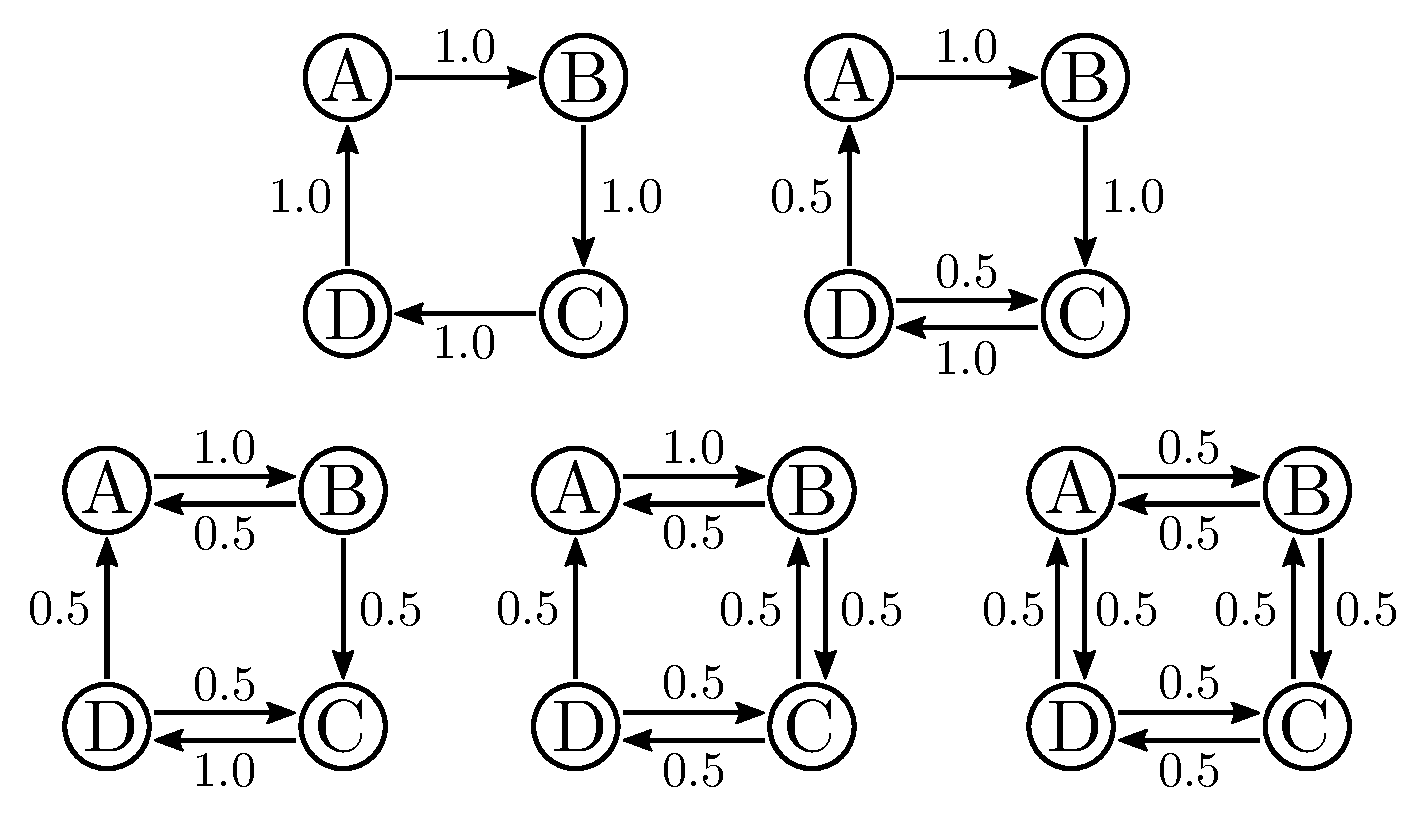
\includegraphics[width=0.85\textwidth]{results/mc1_models}
	\caption[First Markov models]{The first $4$ state Markov models, denoted as model series I. Starting point is a periodic Markov chain, where from model to model one more state is split with a probability of $p_{ij} = 0.5$. The models are enumerated from left to right and from top to down from $1$ to $5$.}
	\label{fig:mc1-models}
\end{figure}

Since there are many combinations of possible Markov chains, in the beginning a discrete state space of size $n = 4$ is chosen with $S = \{A,B,C,D\}$. Furthermore $5$ different Markov chains --- called \emph{models} in the following --- were chosen, shown in figure \ref{fig:mc1-models}. The idea was to start from a periodic Markov chain and systematically introduce more and more backward flow with probability of $p_{ij} = 0.5$. It was hypothesized that:

\begin{itemize}
\item A periodic Markov chain should be learned easily.
\item The more states having probability backward, the harder it can be learned.
\end{itemize}

\paragraph{Performance}

\begin{table}[!b]
\centering
\begin{tabular}{c|ccccc}
Model & 2 & 3 & 4 & 5 \\
\hline
\multirow{2}{*}{1} & $1.303\cdot 10^{-20}$ & $1.803\cdot 10^{-19}$ & $4.656\cdot 10^{-13}$ & $\mathbf{0.986}$ \\
 & ($18.51$) & ($17.14$) & ($10.73$) & ($0.02$) \\
\hline
\multirow{2}{*}{2} & & $1.561\cdot 10^{-05}$ & $1.099\cdot 10^{-15}$ & $8.475\cdot 10^{-21}$ \\
& & ($4.95$) & ($13.12$) & ($18.75$) \\
\hline
\multirow{2}{*}{3} & & & $6.310\cdot 10^{-12}$ & $8.091\cdot 10^{-20}$ \\
& & & ($9.78$) & ($17.55$) \\
\hline
\multirow{2}{*}{4} & & & & $6.284\cdot 10^{-14}$ \\
& & & & ($11.49$) \\
%\hline
\end{tabular}
\vspace{5pt}
\caption[p-values of performance differences between Markov models]{$p$-values of transition performance differences between Markov models. The upper value is the $p$-value, the lower value in brackets is the $T$ value. Obviously all values are highly significant, except the bold value which represents the $p$-value of the performance difference between model $1$ and $5$.}
\label{tb:mc1-t-test}
\end{table}

\begin{figure}[p]
    \centering
    \begin{subfigure}{0.48\textwidth}
    	\centering
        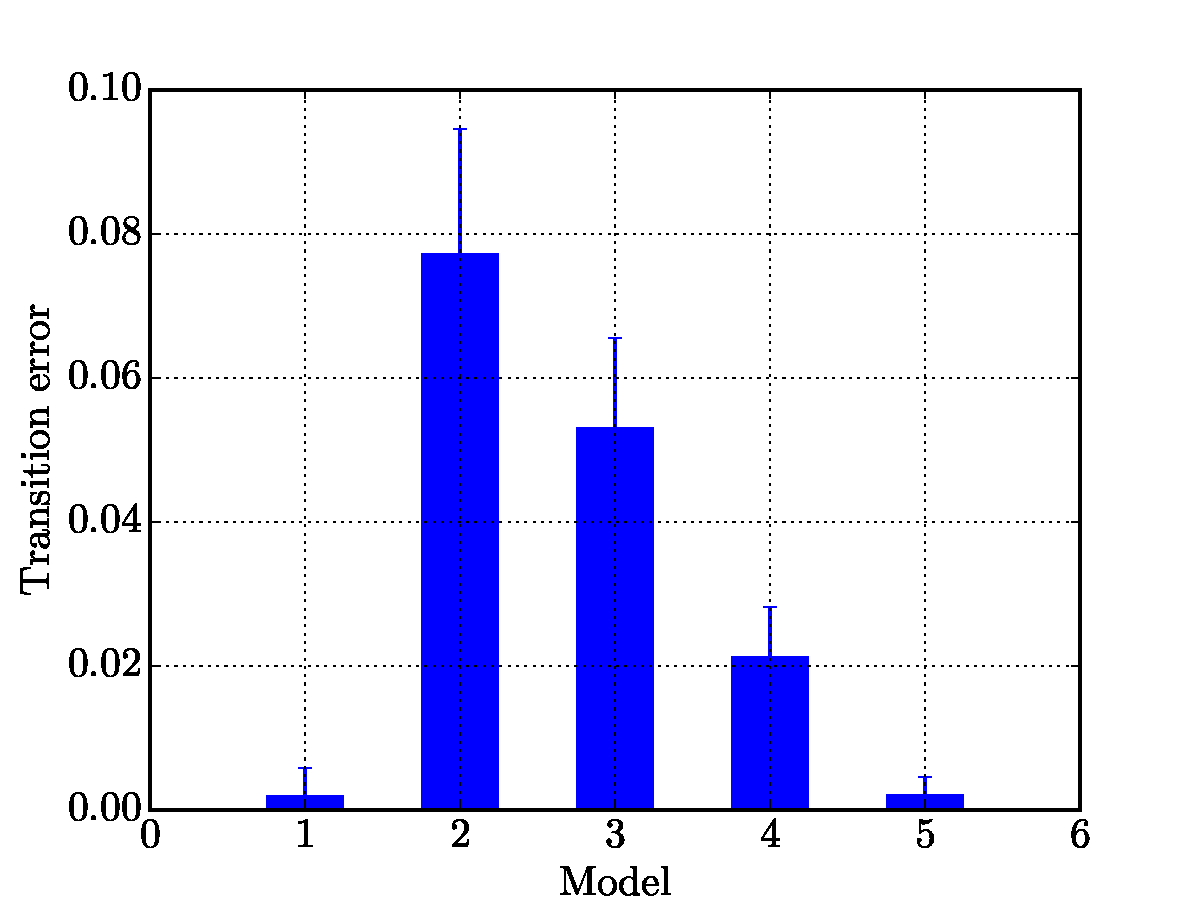
\includegraphics[width=\textwidth]{results/mc1_performance_distances}
        \caption{}
        \label{fig:mc1-performance-transition}
    \end{subfigure}
    \hfill
    \begin{subfigure}{0.48\textwidth}
    	\centering
        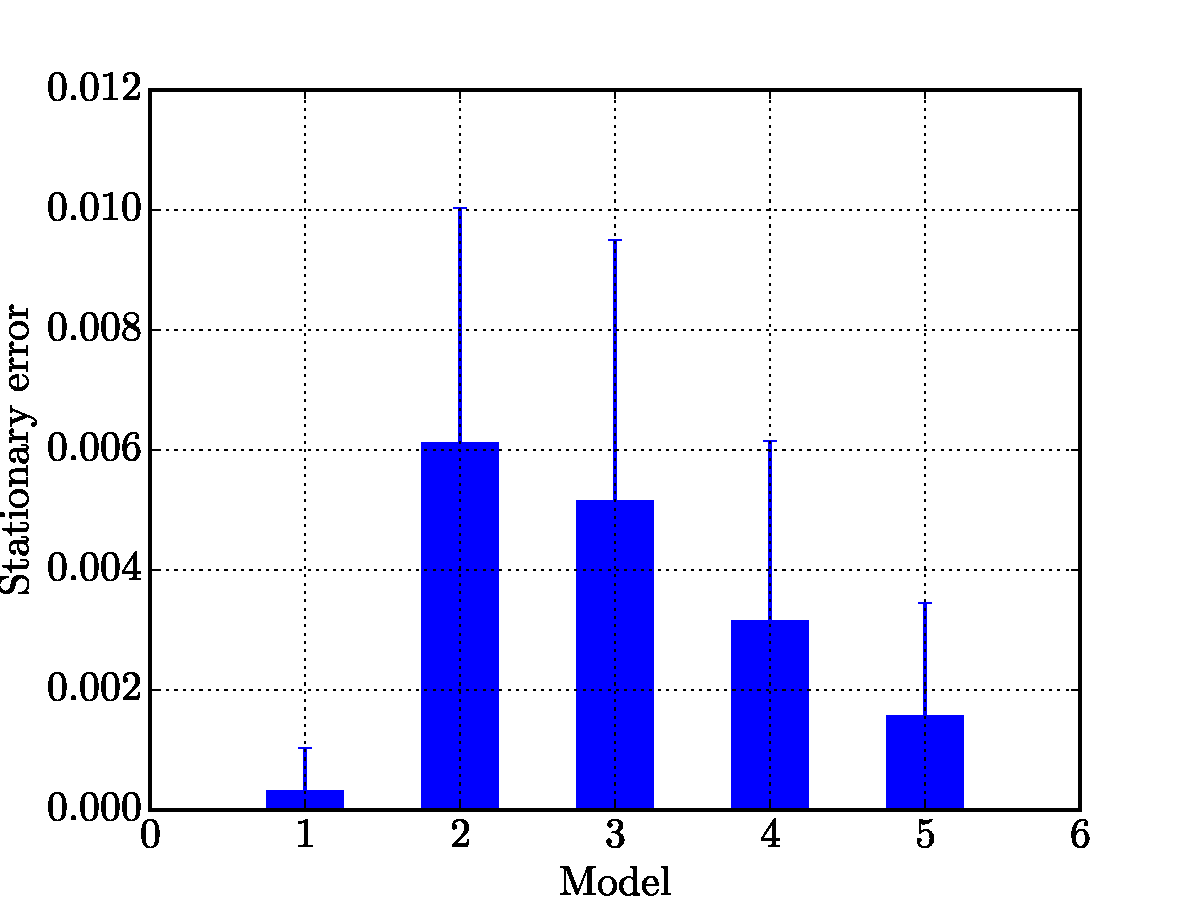
\includegraphics[width=\textwidth]{results/mc1_performance_stationary}
        \caption{}
        \label{fig:mc1-performance-stationary}
    \end{subfigure}
    \begin{subfigure}{0.48\textwidth}
    	\centering
        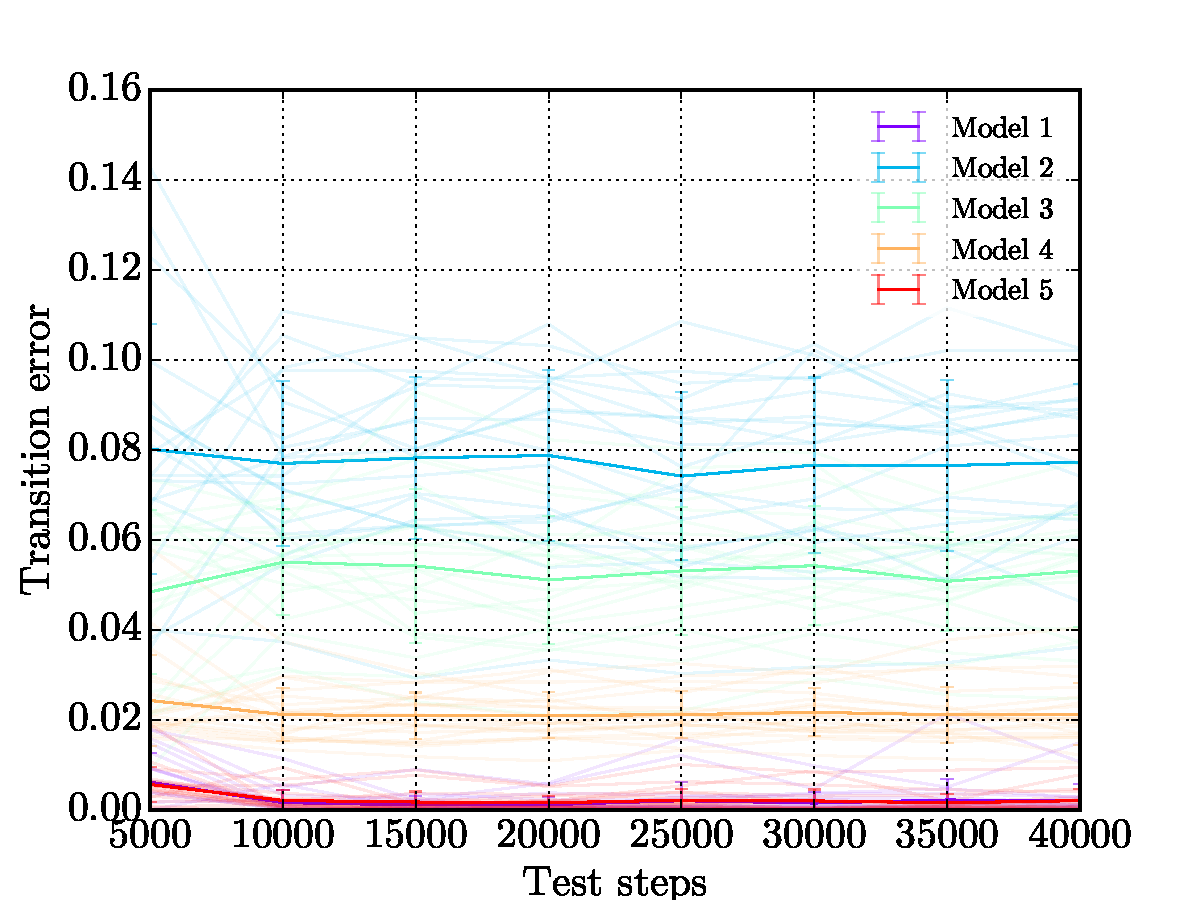
\includegraphics[width=\textwidth]{results/mc1_test_traces_distances}
        \caption{}
        \label{fig:mc1-test_traces-transition}
    \end{subfigure}
    \hfill
    \begin{subfigure}{0.48\textwidth}
    	\centering
        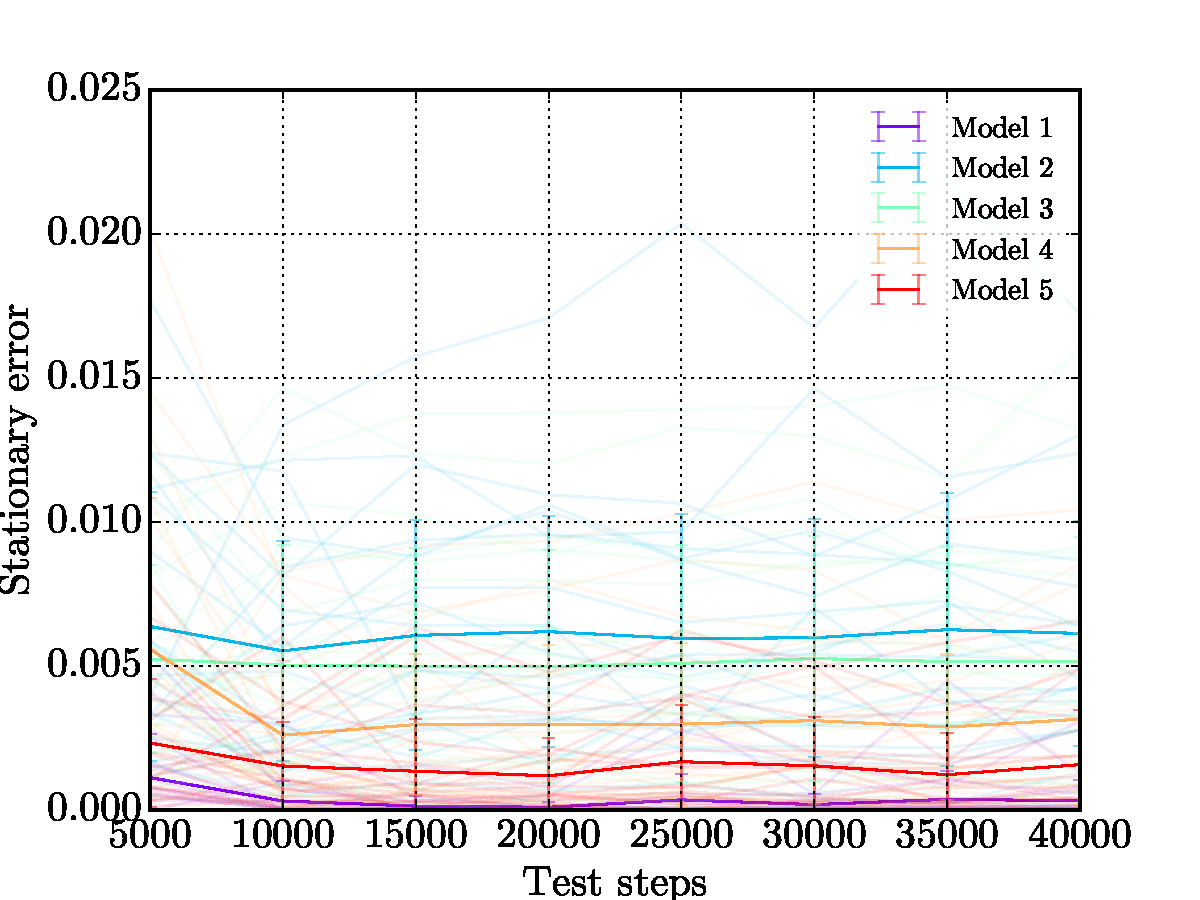
\includegraphics[width=\textwidth]{results/mc1_test_traces_stationary}
        \caption{}
        \label{fig:mc1-test_traces-stationary}
    \end{subfigure}
    \caption[Performance of first Markov models]{Performance of first Markov models. The transition error $\varepsilon_M$ of the first and last model is very low, as can be seen in in \textbf{a)}. The same holds for the stationary error $\varepsilon_\pi$ in \textbf{b)}. The error bars in \textbf{a)} and \textbf{b)} indicate standard errors. The $\varepsilon_M$ and $\varepsilon_\pi$ correspond to the last chunk in the testing phase. The error over all chunks in the testing phase is shown in \textbf{c)} and \textbf{d)}.}
    \label{fig:mc1-performance}
\end{figure}

In figures \ref{fig:mc1-performance-transition} and \ref{fig:mc1-performance-stationary} the performance of the $5$ models is shown. While the first hypothesis is true, the periodic Markov chain can be learned with high performance, the second hypothesis is not true. There is no relation between the number of backward directions and the performance. Furthermore, the performance differences between the models seem high. Results of t-tests show that all models differ highly significant with $p < 0.0001$ in transition performance $\varepsilon_M$, except between model $1$ and $5$ where $p=0.986$, where the null hypothesis cannot be rejected. Table \ref{tb:mc1-t-test} shows the results of all t-test pairs. An example for a learned transition matrix is shown in table \ref{tb:mc1-example}.

Additionally the performance over time was plotted in figures \ref{fig:mc1-test_traces-transition} and \ref{fig:mc1-test_traces-stationary}, showing that the performance is stable over time in testing phase. This is reasonable, since \acl{stdp} is not active in testing phase and the weights stay constant. To prove that \acs{stdp} is the cause for the stable behavior, another simulation was done in appendix \ref{sec:appendix:stdp}, where \acs{stdp} was switched on in the testing phase. And indeed, the information is lost by time and the network `forgets' if \acs{stdp} is active and the weights are still plastic. Furthermore, after the first testing chunk from $5,000$ to $10,000$ steps, there is a slight drop in error. This is due to a burn in phase, which depends on $\eta_\IP$. It takes some time until the spontaneous activity reaches a stable state. Details regarding the burn in phase are given in appendix \ref{sec:appendix:eta}.

\begin{table}[!b]
\centering
\begin{tabular}{ccccc}
\multicolumn{5}{c}{Initial transition} \\
\hline
& $A$ & $B$ & $C$ & $D$\\
$A$ & $0$ & $1.0$ & $0$ & $0$ \\
$B$ & $0.5$ & $0$ & $0.5$ & $0$ \\
$C$ & $0$ & $0.5$ & $0$ & $0.5$ \\
$D$ & $0.5$ & $0$ & $0.5$ & $0$
\end{tabular}
\qquad
\begin{tabular}{ccccc}
\multicolumn{5}{c}{Learned transition} \\
\hline
& $A$ & $B$ & $C$ & $D$\\
$A$ & $0.02$ & $\mathbf{0.75}$ & $0.02$ & $0.21$ \\
$B$ & $\mathbf{0.48}$ & $0.04$ & $\mathbf{0.47}$ & $0.01$ \\
$C$ & $0.02$ & $\mathbf{0.61}$ & $0.03$ & $\mathbf{0.34}$ \\
$D$ & $\mathbf{0.46}$ & $0.05$ & $\mathbf{0.48}$ & $0.01$
\end{tabular}
\vspace{5pt}
\caption[Example for a learned transition matrix]{Example for a learned transition matrix. On the left side, model $4$ is shown. The transition probabilities were used to train the network. On the right side, the learned transition matrix of model $4$ is shown. The probabilities are calculated using equation \eqref{eq:transition-estimation}. Bold values were initially non-zero. While most transitions are represented quite well by the network, the transition from $A$ to $B$ differs a lot.}
\label{tb:mc1-example}
\end{table}

In conclusion, the main interesting effect is that the models seem to perform differently and there is currently no explanation why they behave in that way. It is striking, that model $1$ and $5$ seem very simple. Model $1$ represents just a deterministic input pattern and \textcite{hartmann2015s} already showed that such an input is represented quite well in the network. On the other hand, model $5$ has kind of a `random' structure. Except connections between $A$ \& $C$ and $B$ \& $D$, everything else has no strong restrictions, whereas the other models have more restrictions. For example model $4$: If the network reaches state $A$, it can only change to state $B$, which is a strong restriction, since all the other transitions are allowed to change to two directions. The results, shown in table \ref{tb:mc1-example}, seem to support this explanation. It seems to be problematic to learn the connection between $A$ and $B$, a lot of probability is `lost' in this row.

The mean squared error from the transition matrix seems to be a sufficient measure. It is able to reflect the performance of the network and captures more information than the stationary distribution. Hence, in the following, only the performance measures obtained from the transition matrices  $\varepsilon_M$ are shown.

\paragraph{Plastic training}

\begin{figure}[!b]
	\centering
	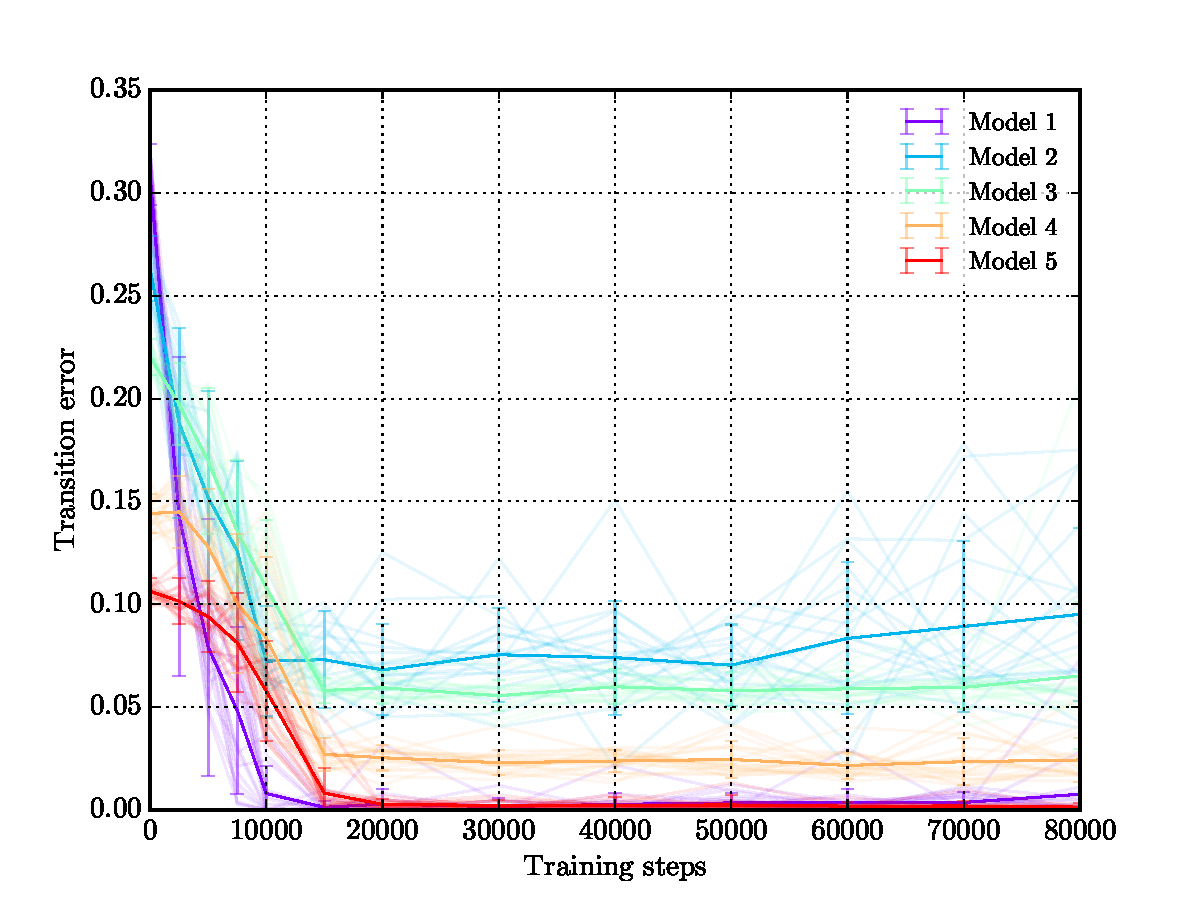
\includegraphics[width=0.95\textwidth]{results/mc1_distances_training_steps_transition}
	\caption[Influence of training to first Markov models]{Influence of training to first Markov models. The transparent lines are all $\Nsim=20$ simulations per model. The opaque lines represent the error $\varepsilon_M$ of a model per line for all simulations. Error bars indicate the standard error. Up to $T_\plastic = 20,000$ the steps were increased by $5,000$, after that, they were increased in steps of $10,000$. Model $1$ and $5$ saturate earlier than the other models, but finally all models reach a specific performance level and do not approximate each other. Training is not able to explain the performance differences between the models.}
	\label{fig:mc1-training}
\end{figure}

It is very likely that the network performs better if the time for training is increased. If absolutely no plastic training is applied, meaning that $T_\plastic = 0$, the network can be seen as a reservoir network. The weights are initialized, but not adapted to the input in that case. The more steps $T_\plastic$ are chosen, the better the performance should be, due to the \acs{stdp} mechanism. It could be that the $T_\plastic = 50,000$ training steps are not enough for all models. Perhaps, model $2$, $3$ and $4$ need a longer training to perform well. In order to understand the influence of the parameter, $T_\plastic$ was varied from $T_\plastic = 0$ to $T_\plastic = 80,000$. There are three hypothesis regarding the plastic training phase:

\begin{itemize}
\item All models improve in performance when training is extended and the performance increase is decreasing, the longer the training is conducted.
\item Different models need different self-organizing time for a good performance.
\item The longer the training period is, the closer the models get, regarding their performance.
\end{itemize}

The results in figure \ref{fig:mc1-training} show that the self-organizing phase has an important influence. The first hypothesis is partly true, since the performance increases, when more training is performed. But the increase in performance is saturating after about $T_\plastic \approx 20,000$ steps of plastic training.

Model $1$ and $5$ seem to saturate earlier (at about $T_\plastic \approx 10,000$) than the other models (at about $T_\plastic \approx 15,000$ to $T_\plastic \approx 20,000$). This behavior is in line with the second hypothesis. But since all of them are saturating, it contradicts the third hypothesis. At which point the network saturates, seems to depend slightly on the model, but still the previous differences remain after all. Differences in the length of the plastic training phase are not able to explain performance differences between models.

\paragraph{Size of the network and size of input cluster}

It is necessary to develop further ideas why the models have different performance in the same network. Another idea is to check the size of the network. It could be that --- for some reason --- some models need more neurons to find a good representation. It is important to also control the number of input connections to the network. If the network size is increased, but the number of connections between input neurons and excitatory neurons stays constant, it could be that the input information has too little influence, compared to ongoing spontaneous activity. In case of small input clusters, most of the network would just end up in spontaneous activity. Therefore, both parameters were varied at the same time. The network size was tested between $N^E = 100$ and $N^E = 500$ in steps of $\Delta N^E = 50$ and the number of input connections varied from $N^U_{x_i} = f_U \cdot N^E = 0.03 \cdot N^E$ to $N^U_{x_i} = 0.15 \cdot N^E$ in steps of $\Delta N^U_{x_i} = 0.01 \cdot N^E$. Since the number of inhibitory neurons depends on the number of excitatory neurons by $N^I = 0.2 \cdot N^E$, also the number of inhibitory neurons are changed.

\begin{figure}[p]
    \centering
    \begin{subfigure}{0.48\textwidth}
    	\centering
        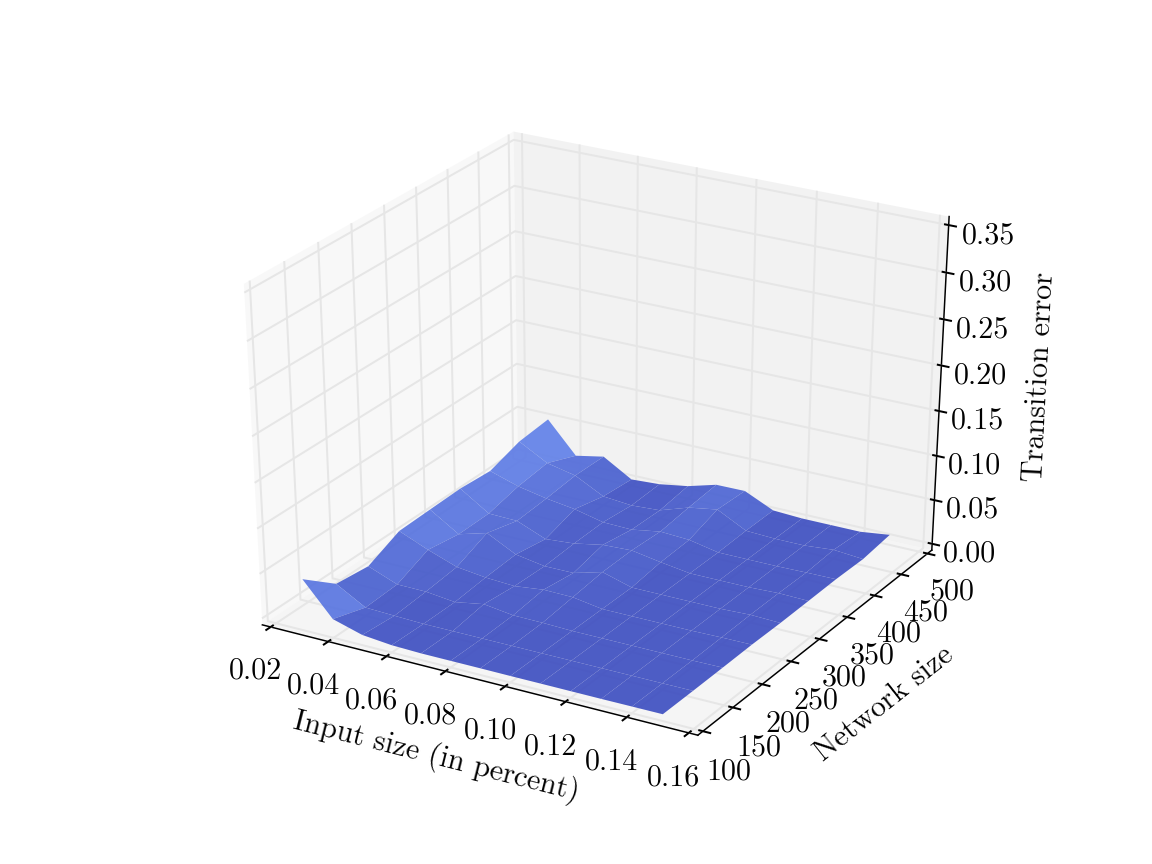
\includegraphics[width=\textwidth]{results/mc1_distances_size_inputs_0}
        \caption{Model $1$}
        \label{fig:mc1-size-0}
    \end{subfigure}
    \hfill
    \begin{subfigure}{0.48\textwidth}
    	\centering
        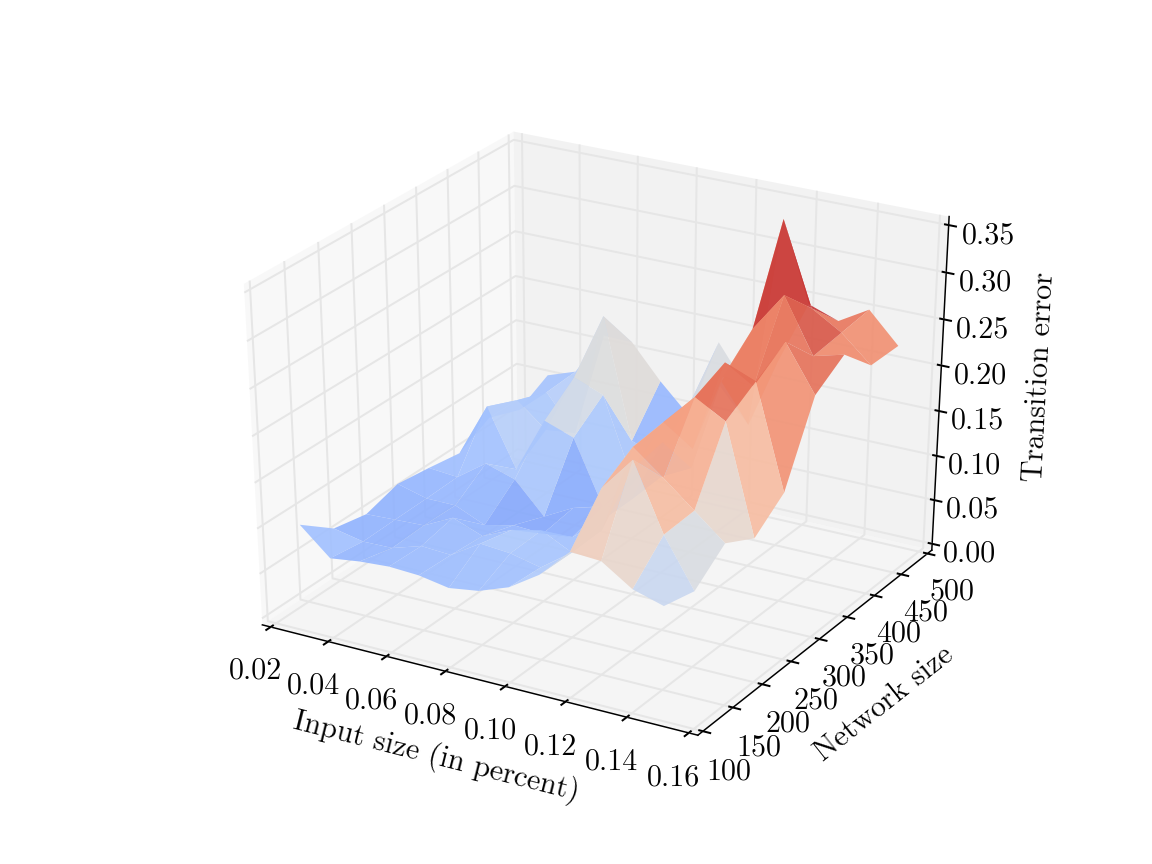
\includegraphics[width=\textwidth]{results/mc1_distances_size_inputs_1}
        \caption{Model $2$}
        \label{fig:mc1-size-1}
    \end{subfigure}
    \begin{subfigure}{0.48\textwidth}
    	\centering
        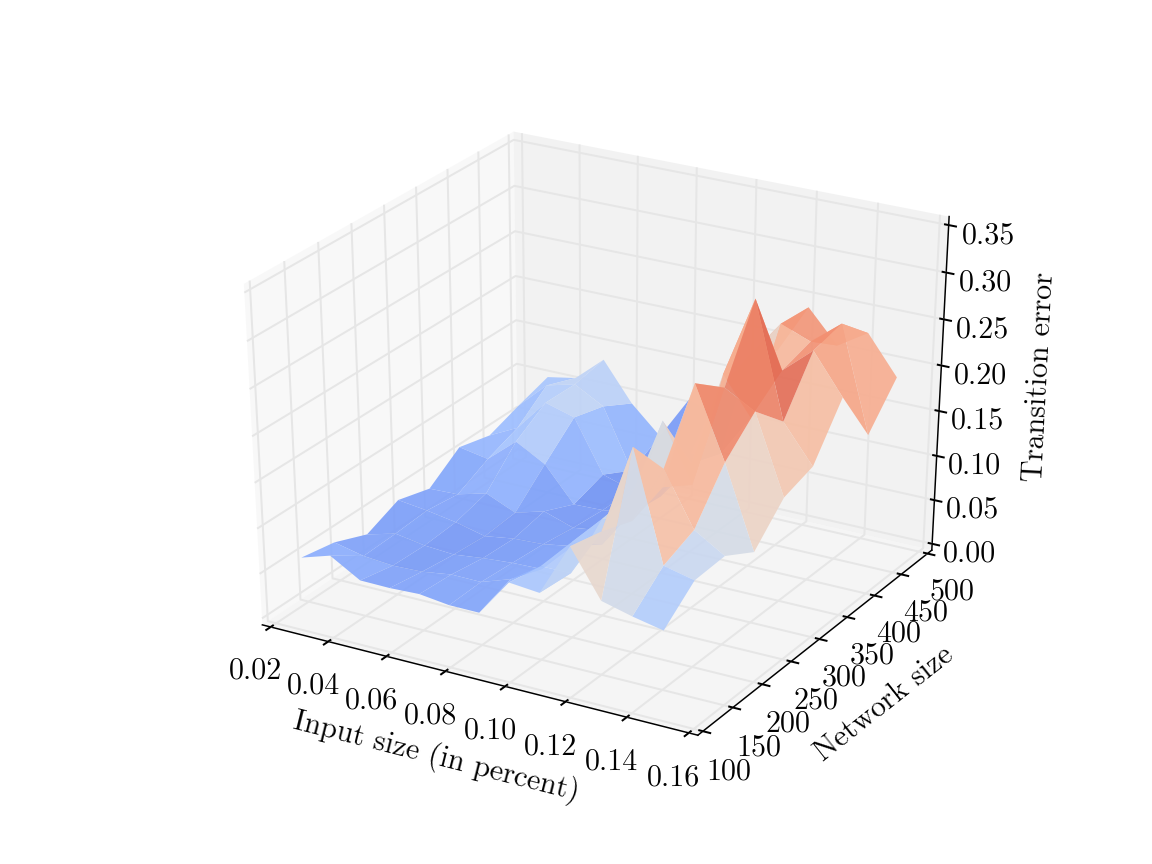
\includegraphics[width=\textwidth]{results/mc1_distances_size_inputs_2}
        \caption{Model $3$}
        \label{fig:mc1-size-2}
    \end{subfigure}
    \hfill
    \begin{subfigure}{0.48\textwidth}
    	\centering
        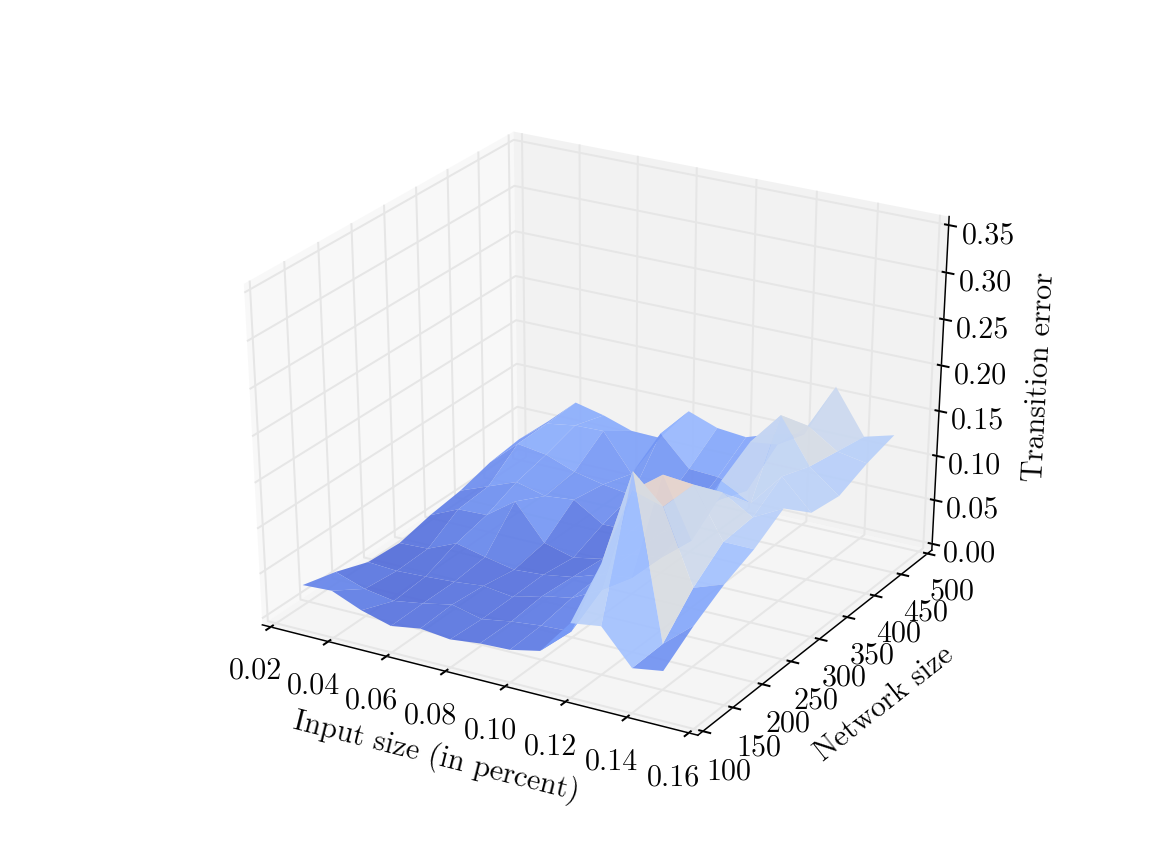
\includegraphics[width=\textwidth]{results/mc1_distances_size_inputs_3}
        \caption{Model $4$}
        \label{fig:mc1-size-3}
    \end{subfigure}
    \begin{subfigure}{0.48\textwidth}
    	\centering
        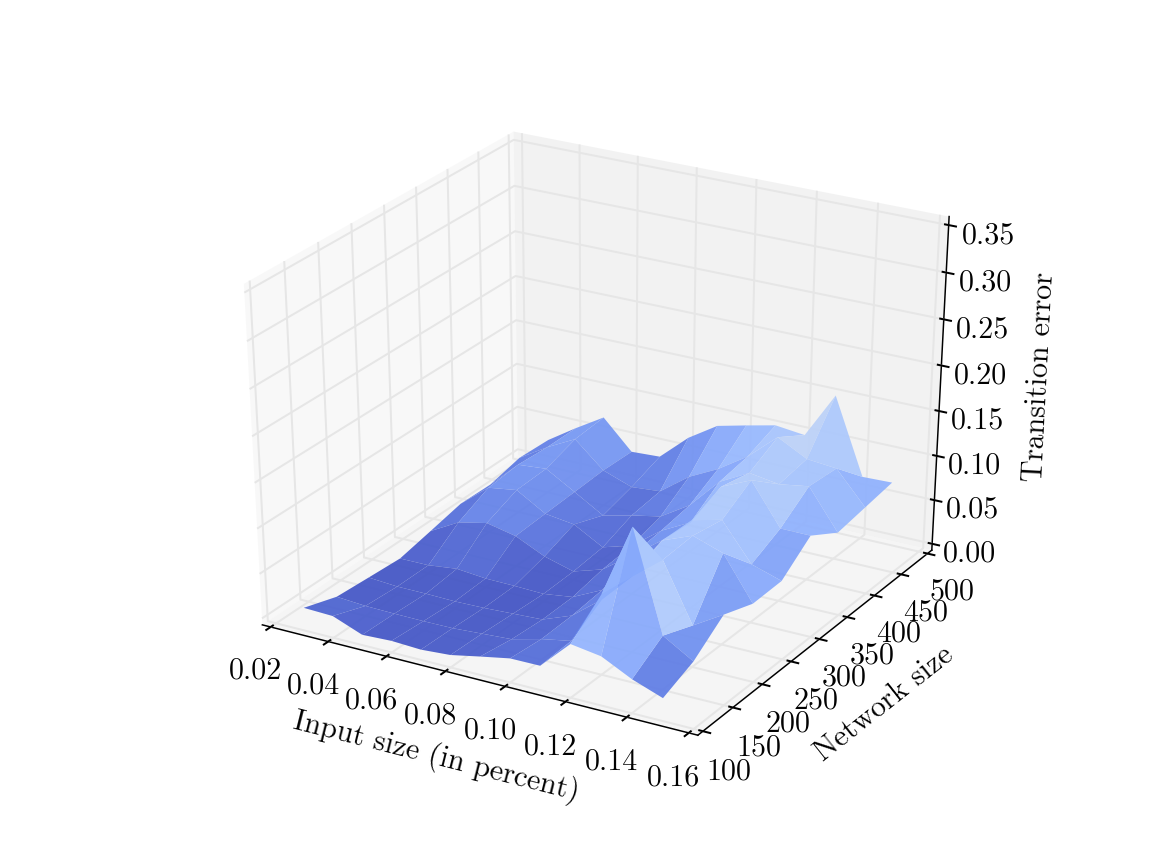
\includegraphics[width=\textwidth]{results/mc1_distances_size_inputs_4}
        \caption{Model $5$}
        \label{fig:mc1-size-4}
    \end{subfigure}
    \hfill
    \caption[Size of the network and size of the input cluster]{Shown is the performance of the $5$ models, depending on the number of excitatory neurons $N^E$ and the size of the input cluster   for every input $N^U_{x_i}$. $N^E$ was chosen from $100$ to $500$ in steps of $\Delta N^E = 50$. The size of the input cluster or equivalently the number of input-to-excitatory weights per input was chosen as a percentage of $N^E$ for every state. It is defined as $N^U_{x_i} = f_U \cdot N^E$, where $f_U$ was chosen between $0.03$ and $0.15$ in steps of $\Delta f_U = 0.01$. The two parameters do not explain the differences between the models.}
    \label{fig:mc1-size}
\end{figure}

In figure \ref{fig:mc1-size} the results are shown. Both parameters have an influence on the performance, but the mean performance is still different for the models. The initial parameters, proposed by \textcite{hartmann2015s}, of $N^E = 200$, $N^U = 0.2 \cdot 200 = 40$ and $N^U_{x_i} = 0.05 \cdot 200 = 10$ seem to have a good performance, compared to the other combinations. There are interesting effects worth to research on. There is a decay in performance for bigger networks, independent of the number of input connections. Furthermore, the performance decreases for more input connections, but the performance becomes better again for $f_U \ge 0.14$. But since the thesis focuses on the performance discrepancies between the different models, no further investigation was done. The main result is that the differences between the models could not be explained by the network size, nor by the size of the input clusters. While the optimal parameter combination is very similar for all models, the models still differ in their scales.

\paragraph{Classification method}

In section \ref{sec:state-classification}, the classification method was introduced. It was already mentioned that the original selection mechanism from \textcite{hartmann2015s}, to find the activity pattern representations $R_\compare$, was changed. The original method was taking the last $\tilde{T}_\compare = 2500$ steps of the no-plastic training phase. While working with the network, a bias in the classification method was found. The number of available comparison steps $T_\compare^\mini$ differed a lot between the models. Perhaps, the classification algorithm is connected to the differences in the performance. While the updated mechanism was already explained in the methods section theoretically, the original and the updated method will be applied to the case of the $5$ models in this section.

\begin{table}[!b]
\centering
\begin{tabular}{c|cccc}
Model & $\pi_A$ & $\pi_B$ & $\pi_C$ & $\pi_D$ \\
\hline
1 & $\frac{1}{4}$ & $\frac{1}{4}$ & $\frac{1}{4}$ & $\frac{1}{4}$ \\
2 & $\frac{1}{6}$ & $\frac{1}{6}$ & $\frac{2}{6}$ & $\frac{2}{6}$ \\
3 & $\frac{1}{4}$ & $\frac{1}{4}$ & $\frac{1}{4}$ & $\frac{1}{4}$ \\
4 & $\frac{2}{7}$ & $\frac{3}{7}$ & $\frac{2}{7}$ & $\frac{1}{7}$ \\
5 & $\frac{1}{4}$ & $\frac{1}{4}$ & $\frac{1}{4}$ & $\frac{1}{4}$
\end{tabular}
\vspace{5pt}
\caption[Stationary distributions of model series I]{Stationary distributions of first Markov models. In models $1$, $3$ and $5$ all states have equal probabilities, in models $2$ and $4$ the probabilities of the states differ.}
\label{tb:mc1-stat}
\end{table}

In models $1$, $3$ and $5$ every state is equally probable, which can be seen by the stationary distribution, provided in table \ref{tb:mc1-stat}. The stationary distributions for all $5$ models were calculated. The states $A$ and $B$ in model $2$ are less equal, than the others. The same holds for state $D$ in model $4$. In the no-plastic training phase, those states will occur less often, which is elaborated in the following. Note that for the calculation of the stationary distribution of model $1$, theorem \ref{th:markov-stat} cannot be applied, since the model is periodic. In that case only theorem \ref{th:irr-rec} can be applied and model $1$ has no limiting distribution.

In average it is expected that every state  occurs $\tilde{T}_\compare \cdot \pi_{x_i}$. If all states have the same probability, it results in $\tilde{T}_\compare / n = 2500 / 4 = 625$ steps for every state in the comparison phase. The calculation leads to $T_\compare^\mini = \min\{ \tilde{T}_\compare^A, \tilde{T}_\compare^B, \tilde{T}_\compare^C, \tilde{T}_\compare^D \} = \min\{ 625, 625, 625, 625 \} = 625$ states in average, which are available as representative states for the classification. This expected number of steps for every state holds for models $1$, $3$ and $5$. But, for example, for model $2$, the state with the lowest probability is state $A$ and $B$ with $\pi_A = \pi_B = 1/6$. Hence, both states are expected to occur in $2500 \cdot 1/6 \approx 417$ cases. In average the number of available steps for every state is given by $T_\compare^\mini = \min\{ 417, 417, 833, 833 \} = 417$. With an analogous calculation it can be shown that for model $4$ only $357$ steps are available to compare with. The number of available samples for classification is nearly half of the available samples, compared to the models where all states are equally probable.

\begin{figure}[!b]
    \centering
    \begin{subfigure}{0.48\textwidth}
    	\centering
        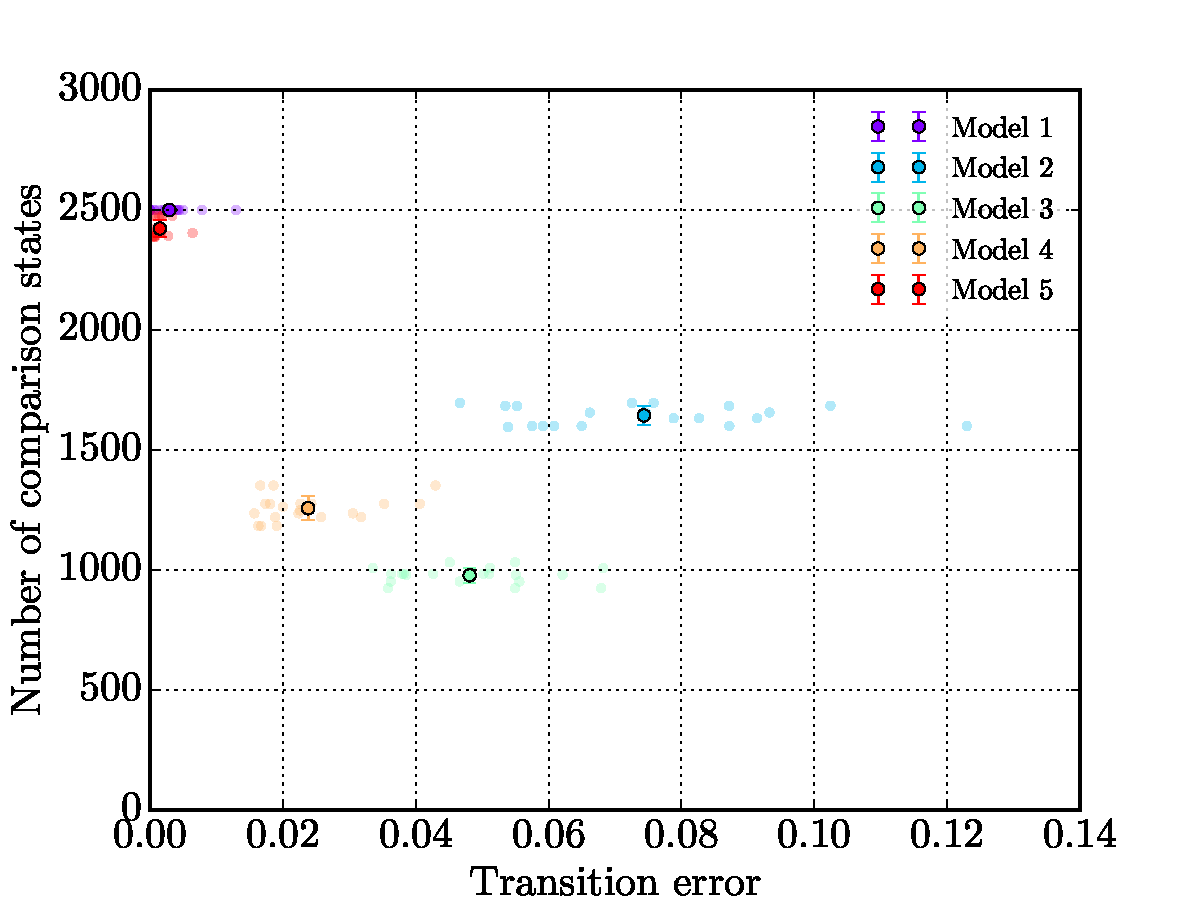
\includegraphics[width=\textwidth]{results/mc1_ncomparison_distances_old}
        \caption{Original method}
        \label{fig:mc1-comparison-old}
    \end{subfigure}
    \hfill
    \begin{subfigure}{0.48\textwidth}
    	\centering
        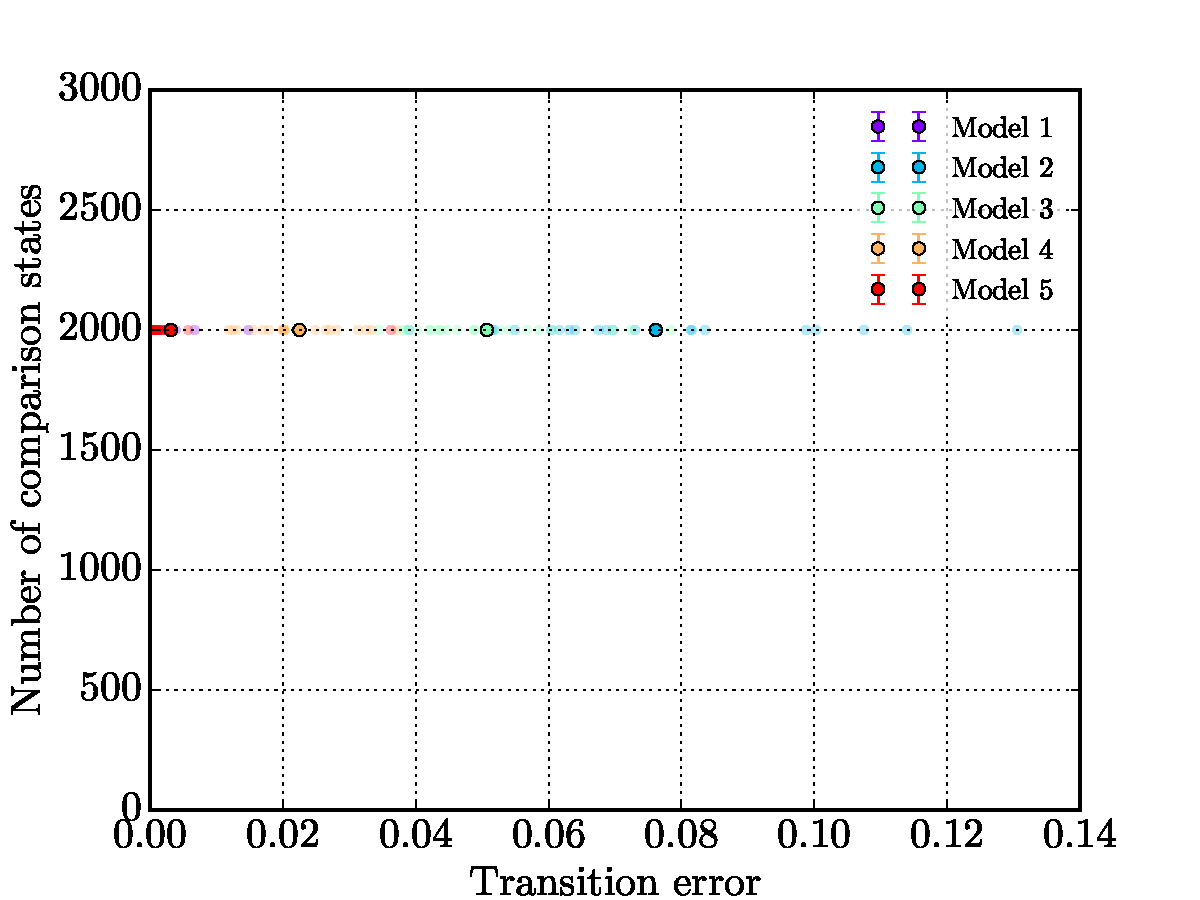
\includegraphics[width=\textwidth]{results/mc1_ncomparison_distances_new}
        \caption{Updated method}
        \label{fig:mc1-comparison-new}
    \end{subfigure}
    \caption[Available steps for comparison]{Available steps for comparison $n\cdot T_\compare^\mini$ with the original method and the updated method in relation to the performance. Transparent points are the single simulations, the opaque points represent their means. Error bars are added for the standard errors of $n\cdot T_\compare^\mini$, but they are very small. The evaluation of the original method is shown in \textbf{a)}. The performance of the transition error seems to depend negative on the transition error, in tendency. Figure \textbf{b)} shows the result if $n\cdot T_\compare$ is fixed. There is no effect by design.}
    \label{fig:mc1-comparison}
\end{figure}

It was hypothesized, that the original selection mechanism influences the performance systematically. There should be a correlation between $T_\compare^\mini$ and the performance $\varepsilon_M$ of the specific model. In figure \ref{fig:mc1-comparison-old} the overall number of available comparison steps $T_\compare^\mini \cdot n$ is shown at the $y$-axis. The error $\varepsilon_M$ is at the $x$-axis. The plot shows that there is indeed a slight negative effect. Of course, there is a ceiling effect since the highest possible $T_\compare^\mini$ is $625$, and therefore also $T_\compare^\mini \cdot n$ has a limit. Additionally, the effect seems not perfectly clear, but still, the correlation is $r_{T\compare} = -0.63$.

The updated mechanism fixes the number of $T_\compare = 500$. An algorithm was searching for the last $500$ representatives for every state in the no-plastic training phase, starting from the end. In that case, independent of the model, the same number of steps is available for classification. The number of necessary no-plastic training $\tilde{T}_\compare$ steps is flexible in that case, which influences the choice of $T_\noplastic$. In the old method the number of no-plastic training steps could easily be estimated, since they never exceeded $\tilde{T}_\compare = 2500$. In the new solution the overall number $\tilde{T}_\compare$ depends on the probability of that state which occurs least. An example was given in section \ref{sec:state-classification}.

The new classification method was also tested. The results with the updated method is shown in figure \ref{fig:mc1-comparison-new}. This time there is no correlation any more, which is expected, since the ceiling is always reached from every model by design. Lastly, the performance measures of all models were compared again with the new method. Surprisingly, even though the correlation is controlled, there is no clear change in the behavior. Hence, there has to be another mechanism responsible for the performance differences between the models. However, the idea to concentrate on the properties of the Markov chain, in terms of the stationary distribution, seemed to be an interesting approach to focus on.

\paragraph{Information of the stationary distribution}

\begin{figure}[!b]
	\centering
	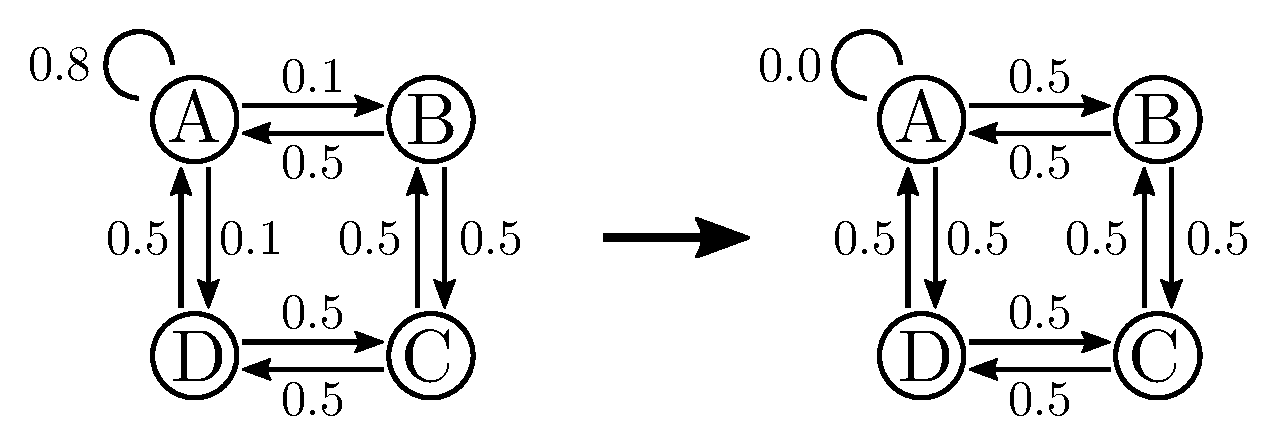
\includegraphics[width=0.85\textwidth]{results/mc2_models}
	\caption[Markov model series II]{Model series II. This time, it is very probable that state $A$ stays in state $A$, whereas $B$, $C$ and $D$ change between each other with equal probability (except $B$ and $D$). Starting from this model, in several steps the probability $p_{AA}$ is decreased to $p_{AA} = 0$ and $p_{AB}$ and $p_{AD}$ are increased to $p_{AB} = p_{AD} = 0.5$. The stationary distributions of all models are shown in table \ref{tb:mc2-stat}.}
	\label{fig:mc2-models}
\end{figure}

In the previous section, the stationary distribution was used to obtain the probabilities for every state. While the research was focused on the parameters of the network only, like the training or size, it would also be possible to focus on the statistical properties of the Markov chain in order to understand what kind of Markov chain can be learned better. In other words, it would be interesting to focus on the properties of the input instead of the network. Since the probabilities indirectly had an effect on the performance in the classification mechanism, it could also be that they directly have an influence. In the previous section, those Markov chains had an influence, where some states had a lower probability than others. This is finally due to a higher variance or due to a higher deviation from the perfectly equally stationary distribution. The latter could be measured by a Kullback-Leibler divergence between a perfectly equally distributed stationary and the present stationary distribution. Both measures were introduced in section \ref{sec:markov-measures}. It is hypothesized that Markov chains with different variance and Kullback-Leibler divergence vary in their performance systematically.

\begin{figure}[p]
    \centering
    \begin{subfigure}{0.48\textwidth}
    	\centering
        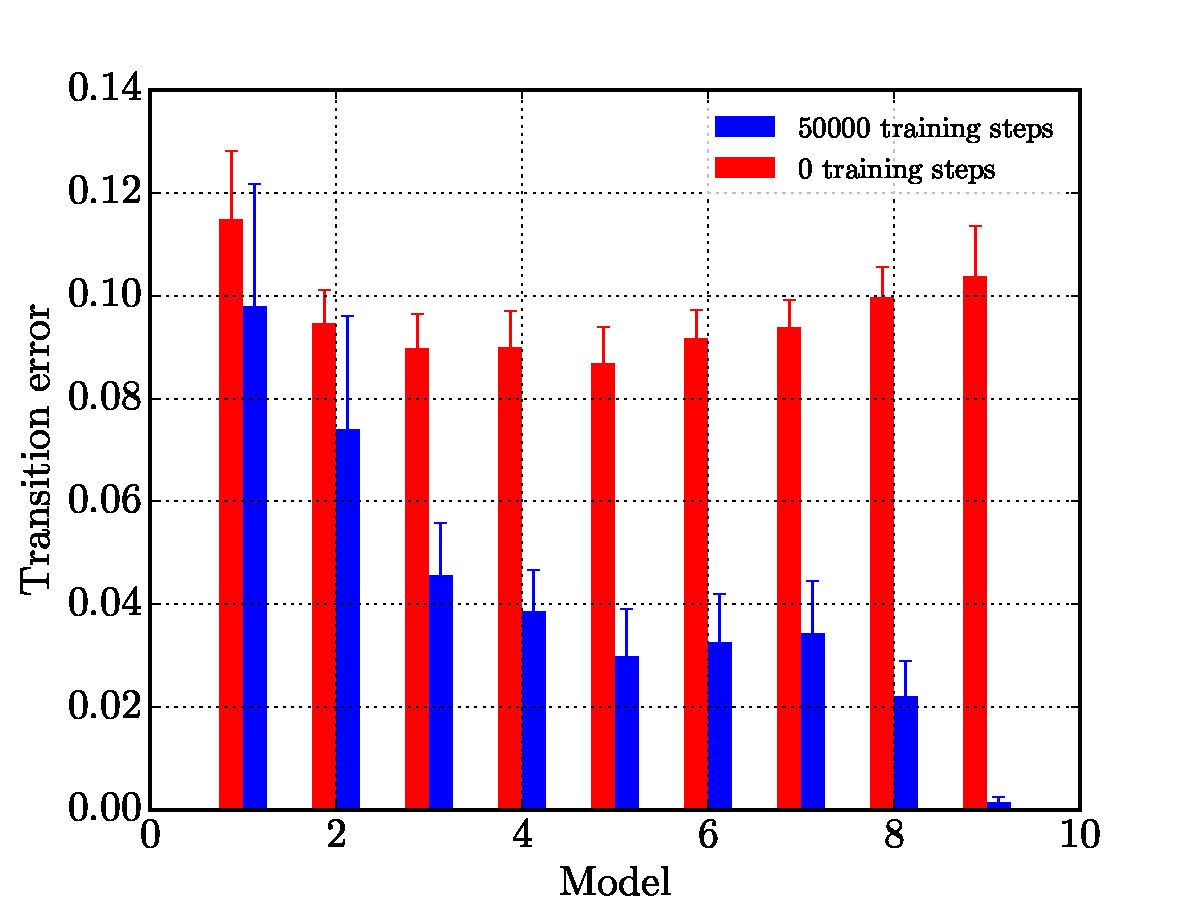
\includegraphics[width=\textwidth]{results/mc2_performance_distances}
        \caption{}
        \label{fig:mc2-performance-distance}
    \end{subfigure}
    \hfill
    \begin{subfigure}{0.48\textwidth}
    	\centering
        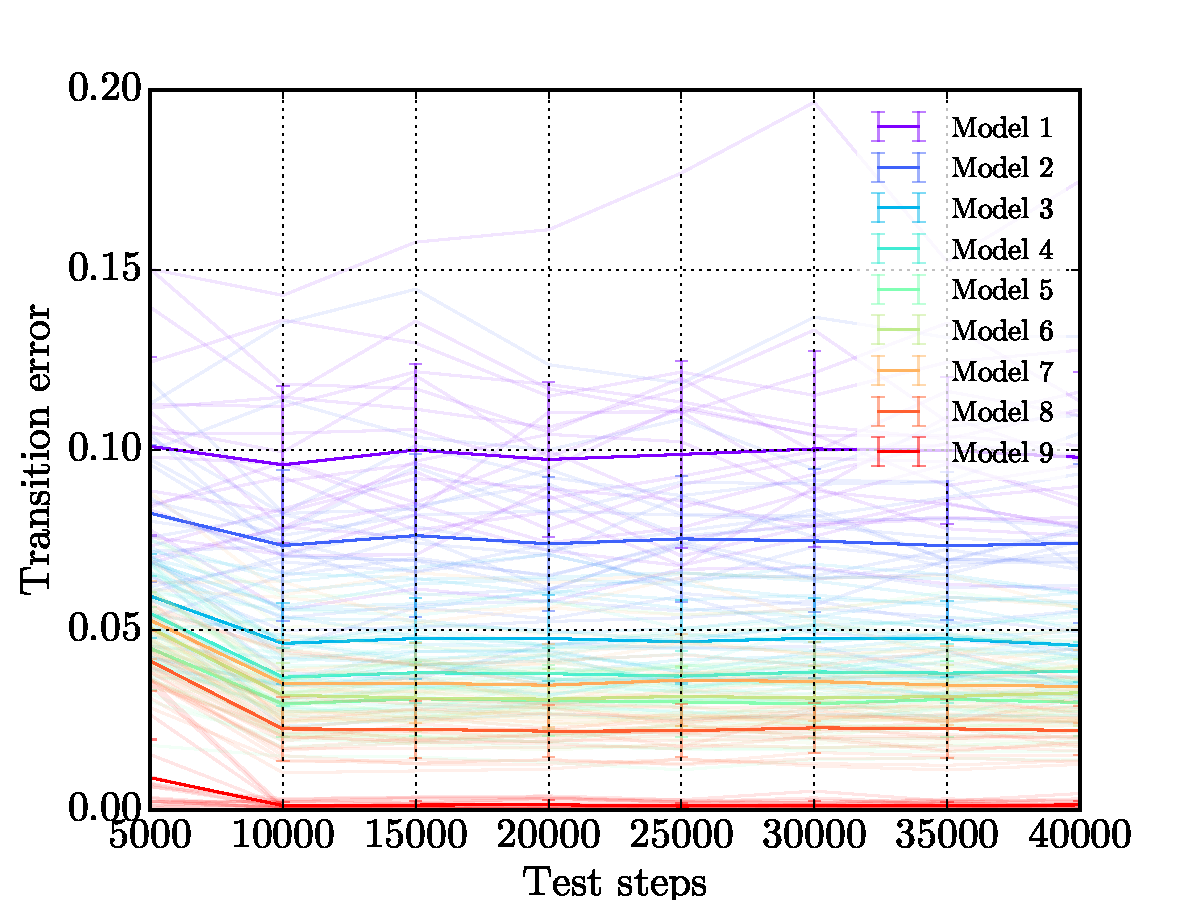
\includegraphics[width=\textwidth]{results/mc2_test_traces_distances}
        \caption{}
        \label{fig:mc2-trace-distance}
    \end{subfigure}
    \begin{subfigure}{0.48\textwidth}
    	\centering
        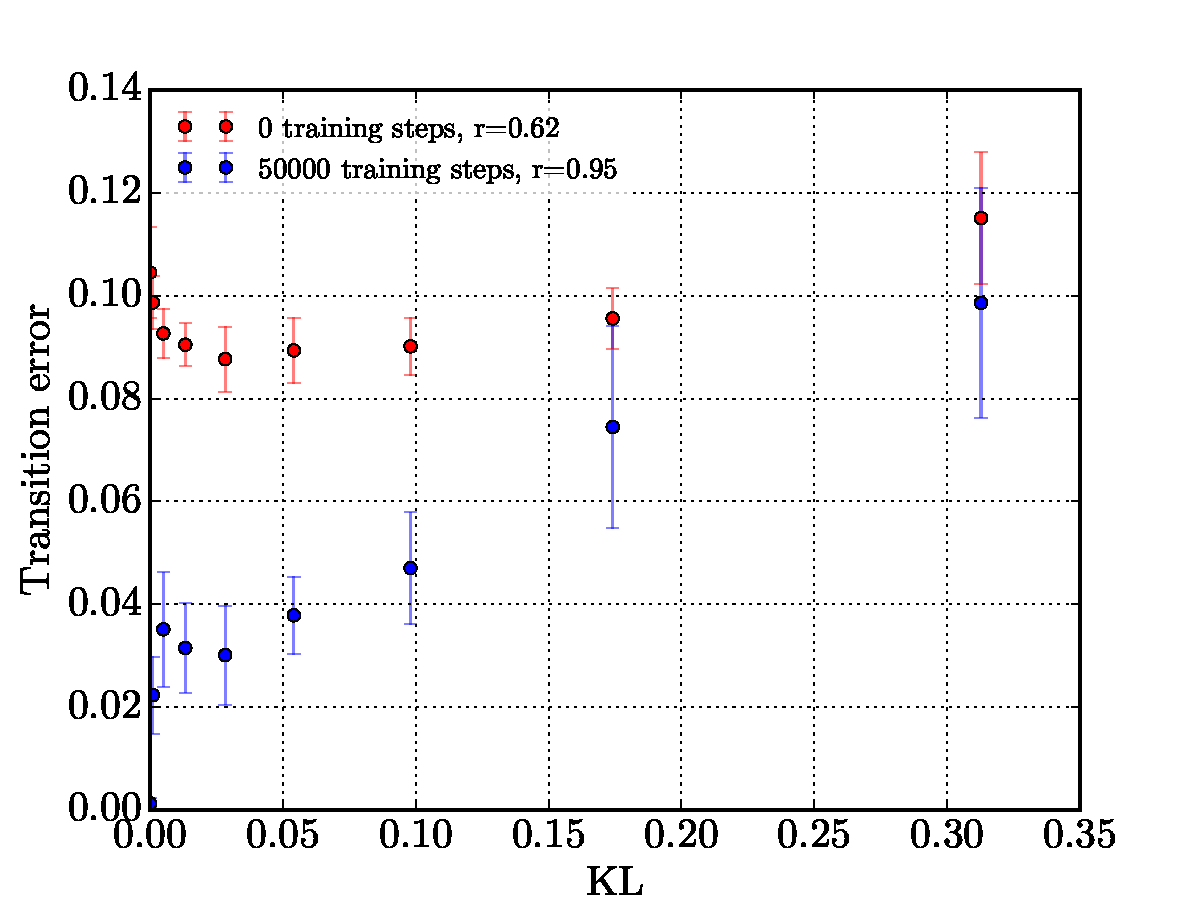
\includegraphics[width=\textwidth]{results/mc2_correlation_inequality_kl_train}
        \caption{}
        \label{fig:mc2-kl}
    \end{subfigure}
    \hfill
    \begin{subfigure}{0.48\textwidth}
    	\centering
        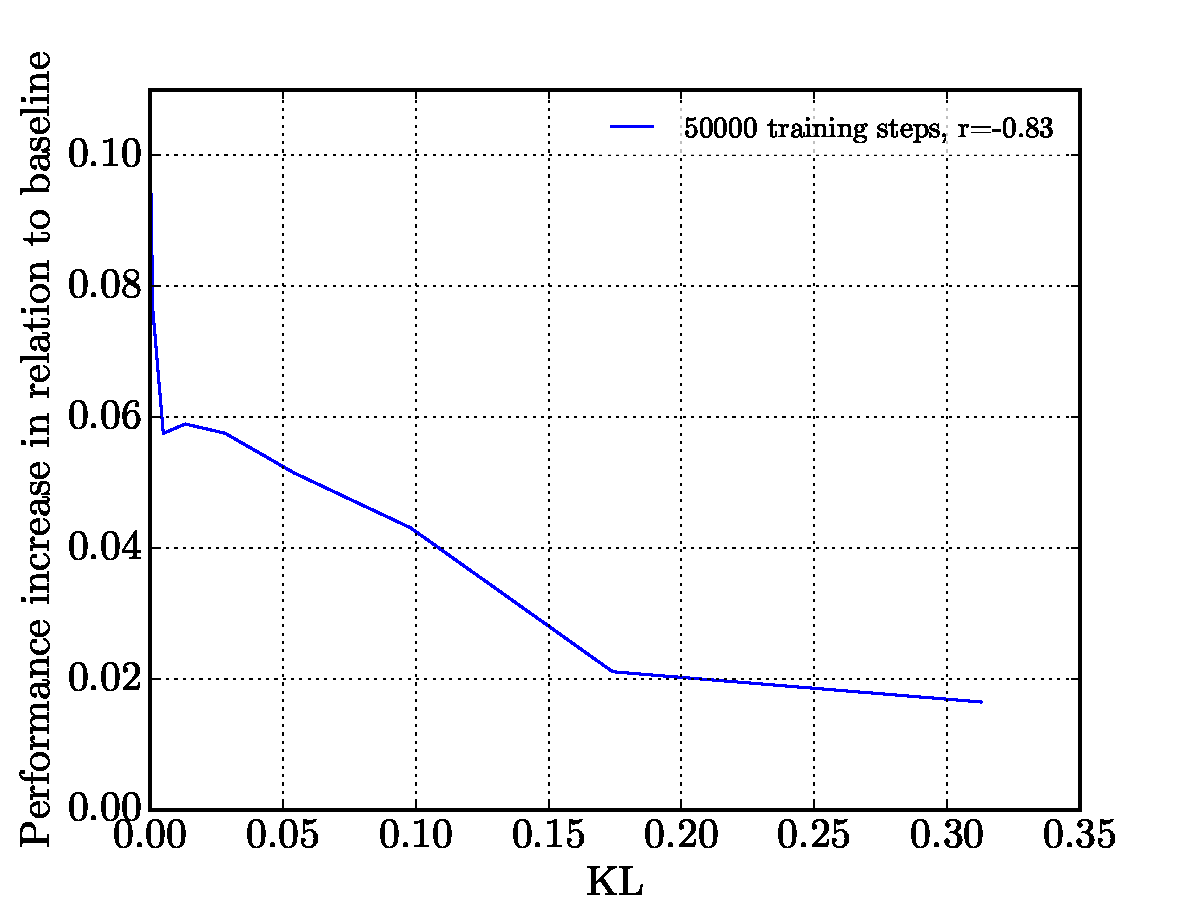
\includegraphics[width=\textwidth]{results/mc2_correlation_inequality_kl_train_baseline}
        \caption{}
        \label{fig:mc2-kl-baseline}
    \end{subfigure}
    \begin{subfigure}{0.48\textwidth}
    	\centering
        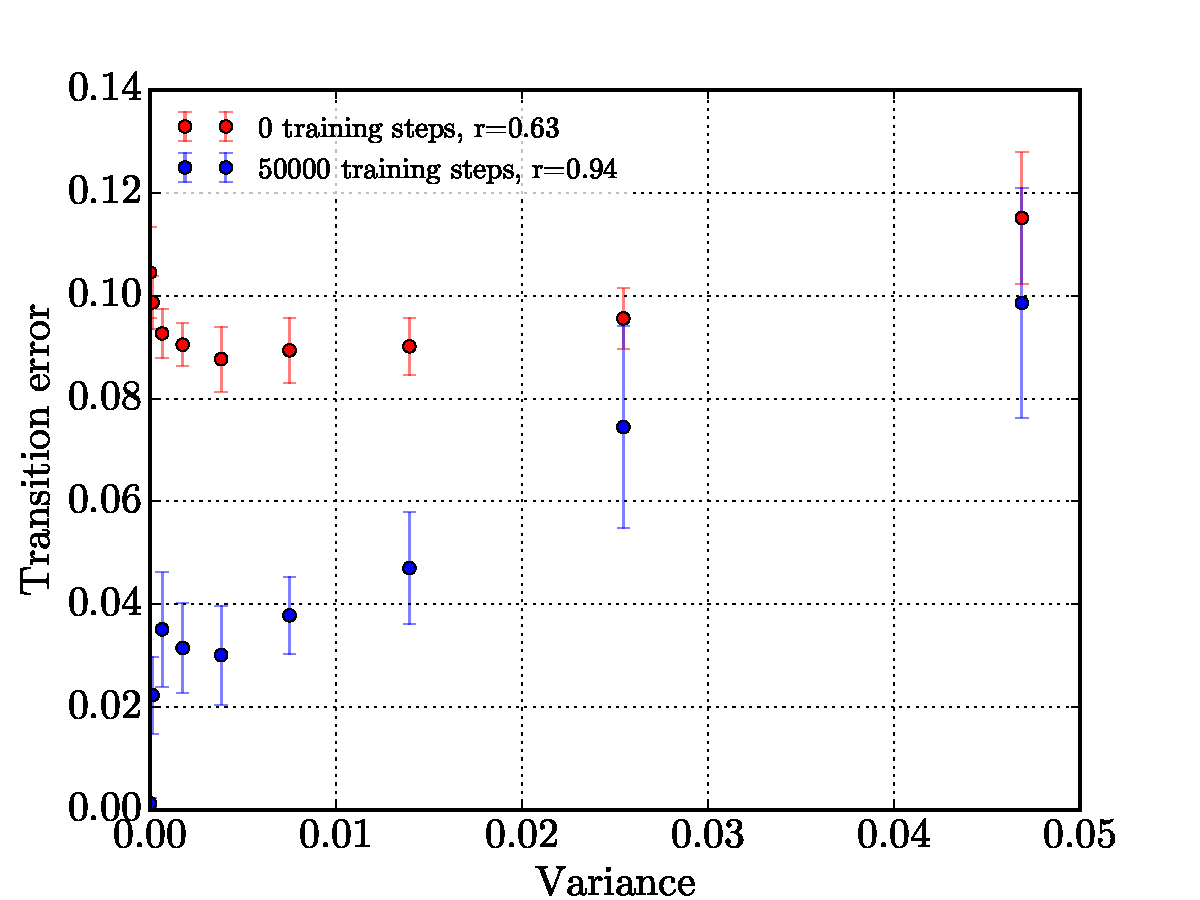
\includegraphics[width=\textwidth]{results/mc2_correlation_inequality_variance_train}
        \caption{}
        \label{fig:mc2-variance}
    \end{subfigure}
    \hfill
    \begin{subfigure}{0.48\textwidth}
    	\centering
        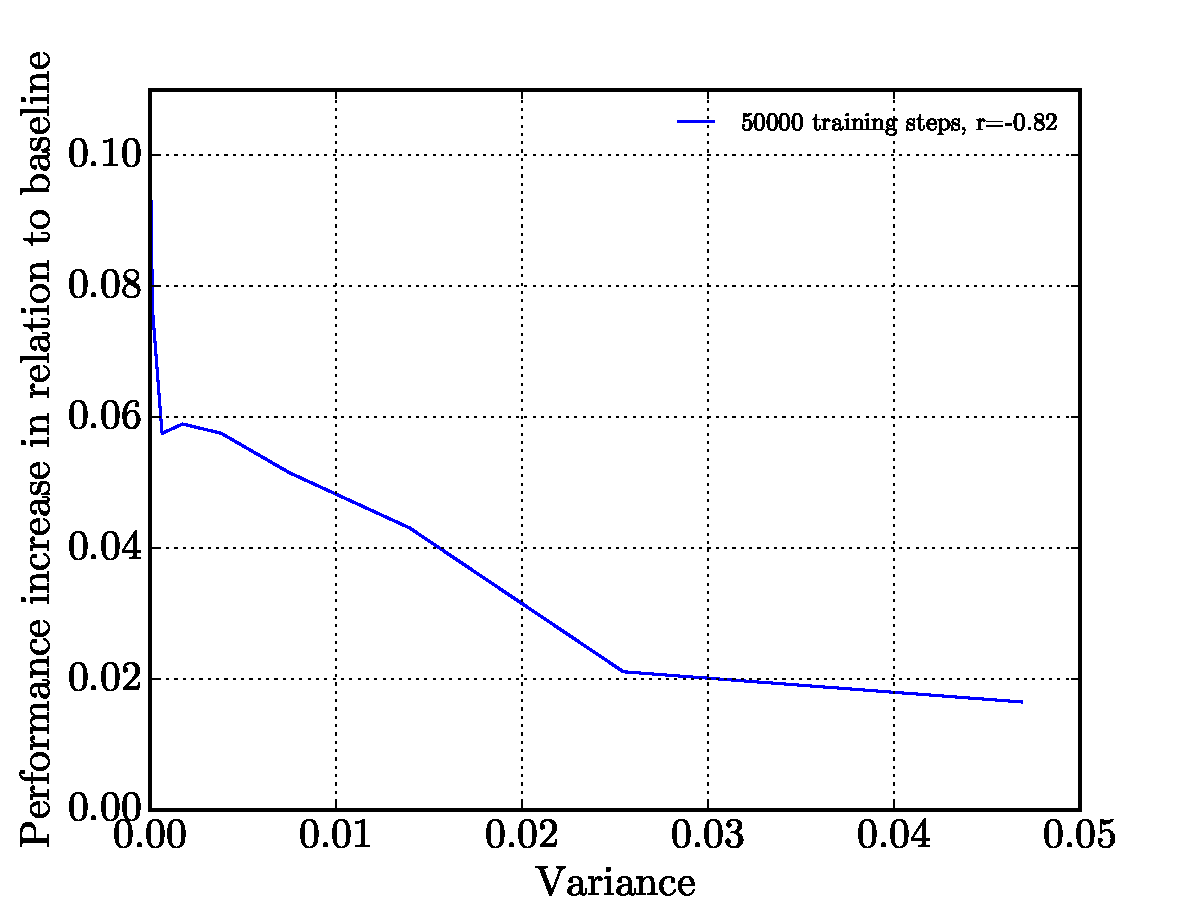
\includegraphics[width=\textwidth]{results/mc2_correlation_inequality_variance_train_baseline}
        \caption{}
        \label{fig:mc2-variance-baseline}
    \end{subfigure}
    \caption[Performance and information of model series II]{Performance and information of model series II. \textbf{a)} shows the performance of the $9$ models. Blue bars show the performance with $50,000$ plastic training steps, red bars with no training, which equals a static reservoir. The performance behavior over the testing phase for the trained network is shown in \textbf{b)} and is constant, as it was expected from previous results. Plot \textbf{c)} shows the correlation between the Kullback-Leibler divergence and the transition error $\varepsilon_M$. Correlations are given in the legend. In \textbf{d)} the increase in performance from the models with $50,000$ plastic training steps in relation to the baseline with $0$ training steps is presented. The correlation is shown in the legend. Plot \textbf{e)} and \textbf{f)} are analog to \textbf{c)} and \textbf{d)} but with the variance of the stationary distribution instead of the Kullback-Leibler divergence.}
    \label{fig:mc2-performance}
\end{figure}

The initially chosen models do not systematically increase the variance $\sigma^2_\pi$ and Kullback-Leibler divergence $\DKL$ in their stationary distribution, which can be seen in table \ref{tb:mc1-stat}. Therefore, a new bunch of models was invented to test the hypothesis. The new models are shown in figure \ref{fig:mc2-models}. The first model has a high probability that state $A$ stays in state $A$, namely $p_{AA} = 0.8$. The probability to leave $A$, $p_{AB}$ and $p_{AD}$, is very small in the first model. Model by model $p_{AA}$ decreases and $p_{AB}$ as well as $p_{AD}$ increase until all transitions have the same probability. The stationary distribution, variance and Kullback-Leibler divergence are shown in table \ref{tb:mc2-stat} for every model. State $A$ is very probable in the first model, compared to the probability of the other states, and increases the variance of the stationary distribution and the Kullback-Leibler divergence. Model by model it becomes less probable, until all states are equally probable, which results in $\sigma^2_\pi = 0$ and $\DKL = 0$.

\begin{table}[!t]
\centering
\begin{tabular}{c|cccc|cc}
Model & $\pi_A$ & $\pi_B$ & $\pi_C$ & $\pi_D$ & $\sigma^2_\pi$ & $\DKL$ \\
\hline
1 & $0.625$ & $0.125$ & $0.125$ & $0.125$ & $0.047$ & $0.31$ \\
2 & $0.526$ & $0.158$ & $0.158$ & $0.158$ & $0.025$ & $0.17$ \\
3 & $0.455$ & $0.182$ & $0.182$ & $0.182$ & $0.014$ & $0.098$ \\
4 & $0.4$ & $0.2$ & $0.2$ & $0.2$ & $0.0075$ & $0.054$ \\
5 & $0.357$ & $0.214$ & $0.214$ & $0.214$ & $0.0038$ & $0.028$ \\
6 & $0.323$ & $0.226$ & $0.226$ & $0.226$ & $0.0018$ & $0.013$ \\
7 & $0.294$ & $0.235$ & $0.235$ & $0.235$ & $0.0006$ & $0.005$ \\
8 & $0.27$ & $0.243$ & $0.243$ & $0.243$ & $0.0001$ & $0.001$ \\
9 & $0.25$ & $0.25$ & $0.25$ & $0.25$ & $0$ & $0$
\end{tabular}
\vspace{5pt}
\caption[Stationary distributions of model series II]{Stationary distributions of the Markov models from the second approach. Shown is also the variance and the Kullback-Leibler divergence of every stationary distribution.}
\label{tb:mc2-stat}
\end{table}

The performance results are shown in figure \ref{fig:mc2-performance-distance} and \ref{fig:mc2-trace-distance}. The simulation was done with $T_\plastic = 50,000$ plastic training steps and with $T_\plastic = 0$ steps. The latter equals a static reservoir network, since the weights are just randomly initialized and not adapted using \acs{stdp}. Interestingly, the static reservoir network behaves nearly equal for every model, which is opposite to the hypothesis of a systematic influence. On the other hand, the networks, where the weights are trained, show a clear rise in performance, when the stationary distribution becomes more equal. Figure \ref{fig:mc2-trace-distance} shows that the performance of the network stays constant in the testing phase. It reproduces the result from the previous models.

In figure \ref{fig:mc2-kl} the \acs{mse} $\varepsilon_M$ is plotted, depending on $\DKL$. For the static reservoir, there is no clear linear tendency for a relationship. Regarding the trained network, a linear tendency can be seen and the correlation is $r_{D_{KL}} = 0.95$. The same holds for a relation between the performance and the variance of the stationary distribution with a correlation of $r_\sigma = 0.94$, shown in figure \ref{fig:mc2-variance}.

The performance of the static reservoir network seems to be kind of a \emph{baseline}, where training is able to improve the performance as long as the stationary distribution is not too unequal. In figures \ref{fig:mc2-kl-baseline} and \ref{fig:mc2-variance-baseline}, the increase in performance is shown in relation to the information measures. The more equal the stationary distribution, the higher is the gain in performance.

Finally, the relation between $\varepsilon_M$ and $\sigma^2_\pi$ as well as $\DKL$ seems to be non-linear for small variances and small values of Kullback-Leibler divergence. The behavior in that area is evaluated in appendix \ref{sec:appendix:close}.

\paragraph{Concentration of the distribution}

While focusing on the information of the stationary distribution in the previous section, it could also be that the concentration of the distribution plays a major role. The results should be similar, since a high concentration normally also includes an increase in variance.

To quantify the concentration of a distribution, the Lorenz curve can be used, which was introduced in section \ref{sec:markov-measures} and illustrated in figure \ref{fig:lorenz-illustration}. While the Lorenz curve is a qualitative assessment, the Gini coefficient $G$, shown in equation \eqref{eq:gini}, quantifies the concentration.

\begin{figure}[!t]
    \centering
    \begin{subfigure}{0.48\textwidth}
    	\centering
        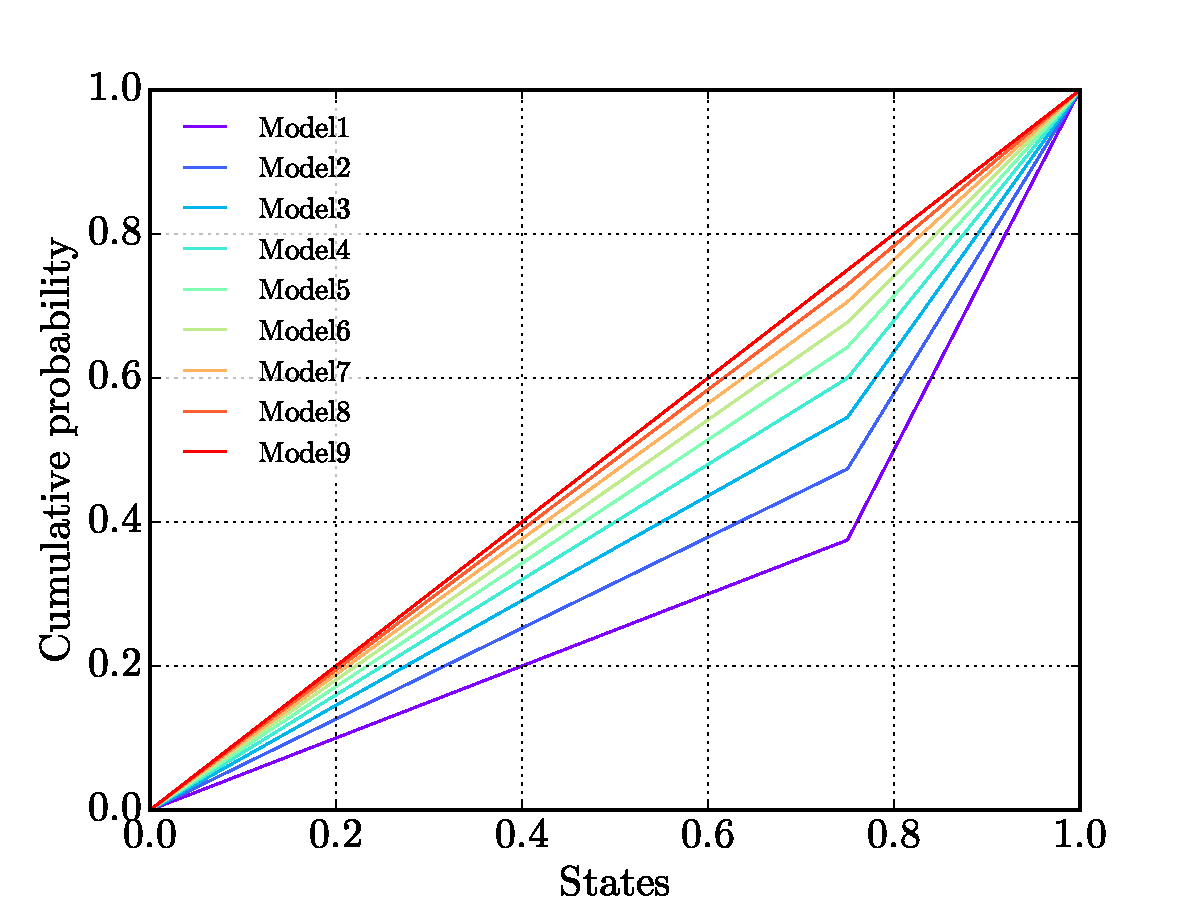
\includegraphics[width=\textwidth]{results/mc2_lorenz-curve}
        \caption{}
        \label{fig:mc2-lorenz}
    \end{subfigure}
    \hfill
    \begin{subfigure}{0.48\textwidth}
    	\centering
        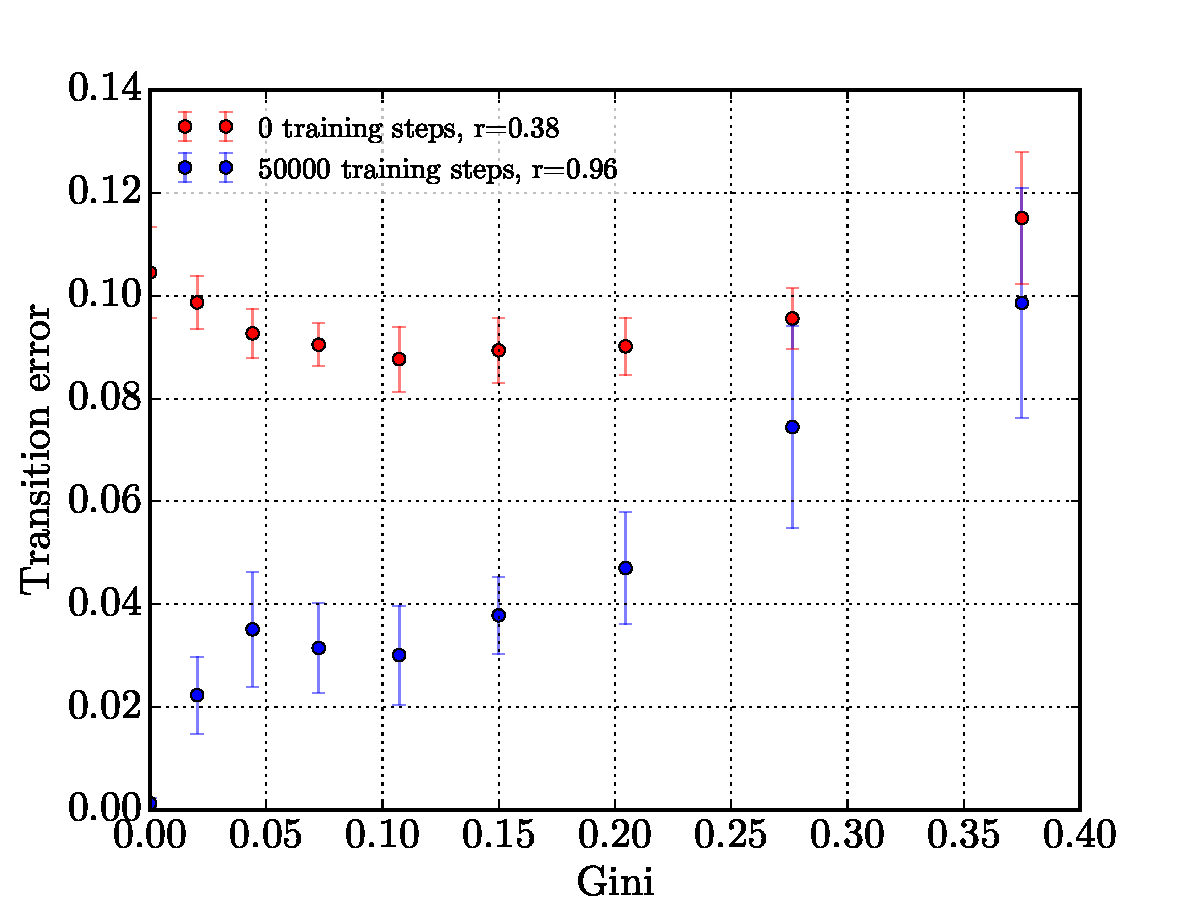
\includegraphics[width=\textwidth]{results/mc2_correlation_inequality_gini_train}
        \caption{}
        \label{fig:mc2-gini}
    \end{subfigure}
    \caption[Concentration of the stationary distribution]{Concentration of the stationary distribution. \textbf{a)} shows the Lorenz curves of all models from the second approach (figure \ref{fig:mc2-models}). The models differ in their concentration. In \textbf{b)} the Gini coefficients are calculated to quantify the concentration measure. They are put in relation with the performance of the models.}
    \label{fig:mc2-concentration}
\end{figure}

Figure \ref{fig:mc2-lorenz} shows the Lorenz curves for the models used above. The amount of concentration obviously differs between the different models. The relation between the performance $\varepsilon_M$ and the Gini coefficient $G$ is shown in figure \ref{fig:mc2-gini}. The effect is quite the same as it was before with the variance and the Kullback-Leibler divergence. Using the Gini coefficient, the correlation is $r_G = 0.96$. Therefore, the concentration of the distribution is just another perspective, but it does not explain more than the former approaches were doing. However, to evaluate the observations under a perspective of concentration had a decisive impact on the idea of the following \acs{ip}-hypothesis.

\subsection{IP-hypothesis}
\label{sec:ip-hyp}

The results from the previous section show a clear relation between the properties of the Markov chain and the performance. It is necessary to develop an explanation for this behavior and it remains to show that this behavior is robust, also for other Markov chains.

The hypothesis, which is suggested to explain the effect, focuses on the \acf{ip}. Therefore, the hypothesis is called \emph{\acs{ip}-hypothesis} in the following. Assume just $3$ states, $A$, $B$ and $C$. They correspond to input clusters at the excitatory neurons. The case is shown in figure \ref{fig:sorn-clusters}. Inhibitory neurons, input neurons and weights are not shown. Further, assume a stationary distribution

\begin{equation}
\pi = (\pi_A, \pi_B, \pi_C)^T = (0.8, 0.1, 0.1)^T.
\end{equation}

A simulation of a Markov chain with such a distribution and the three states could look like

\begin{equation}
A\;A\;A\;A\;A\;A\;A\;C\;B\;A.
\end{equation}

\begin{figure}[!t]
	\centering
	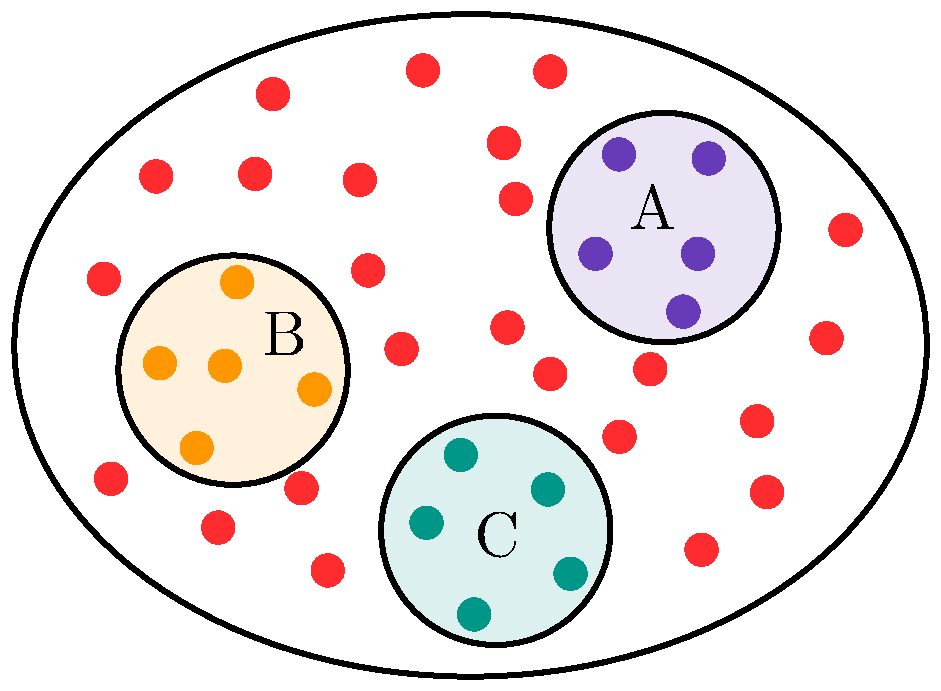
\includegraphics[width=0.65\textwidth]{results/sorn_cluster}
	\caption[Input clusters example]{Three input clusters as an example to illustrate \acs{ip}-hypothesis. If one cluster is not active for a longer time, neurons of that cluster will be active spontaneously and the chance for a misclassification increases.}
	\label{fig:sorn-clusters}
\end{figure}

It is necessary to remind the property of \acs{ip} regarding spontaneous activity, as it was shown in figure \ref{fig:intrinsic-plasticity} in section \ref{sec:ip}. If a neuron is not active for a long time, the threshold of that neuron is going down. If the threshold falls below zero, the neuron fires spontaneously. In the simulation, state $A$ and therefore neuron cluster $A$ is repetitively active in the network for a long time, due to its higher probability $\pi_A$. The threshold of the other neurons is going down at that time, because they are ideally not excited. That affects those neurons of cluster $B$ and $C$ in particular. Therefore, the chance rises that cluster $B$ or $C$ will be active spontaneously after some time.

Models with regular input patterns, meaning that the probabilities of the states are similar, have a better performance than those with irregular input patterns, where some states have a smaller probability than others. The \acs{ip}-hypothesis suggests that \acl{ip} is a cause for that observation. This hypothesis was tested in three steps:

\begin{itemize}
\item Apply different models and evaluate if the effects can be explained by the hypothesis.
\item Vary parameter $\bar H^\IP$ and evaluate if different levels of \acl{ip} influence the performance.
\item Vary parameter $\sigma_\IP$ and evaluate if the performance becomes more robust, independent of the model.
\end{itemize}

\paragraph{More models}

After the effect of the stationary distribution was shown, a bunch of different models was developed to test the \acs{ip}-hypothesis. In figure \ref{fig:mc-models-collection} four series of Markov chains are shown. They were all simulated with $T_\plastic = 50,000$.

The first series in figure \ref{fig:mc3-models}, model series III, is similar to the series of models II, presented in figure \ref{fig:mc1-models}. But while the previous models concentrated their probability at state $A$, in this case the probability is concentrated at states $B$, $C$ and $D$. Therefore, the chance that $A$ will be active spontaneously is increased, since this state is less active than the other states. The performance plot should show similar results to figure \ref{fig:mc2-performance-distance} and indeed, figure \ref{fig:mc3-performance-distance} shows that the results are very similar.

\begin{figure}[p]
    \centering
    \begin{subfigure}{0.85\textwidth}
    	\centering
        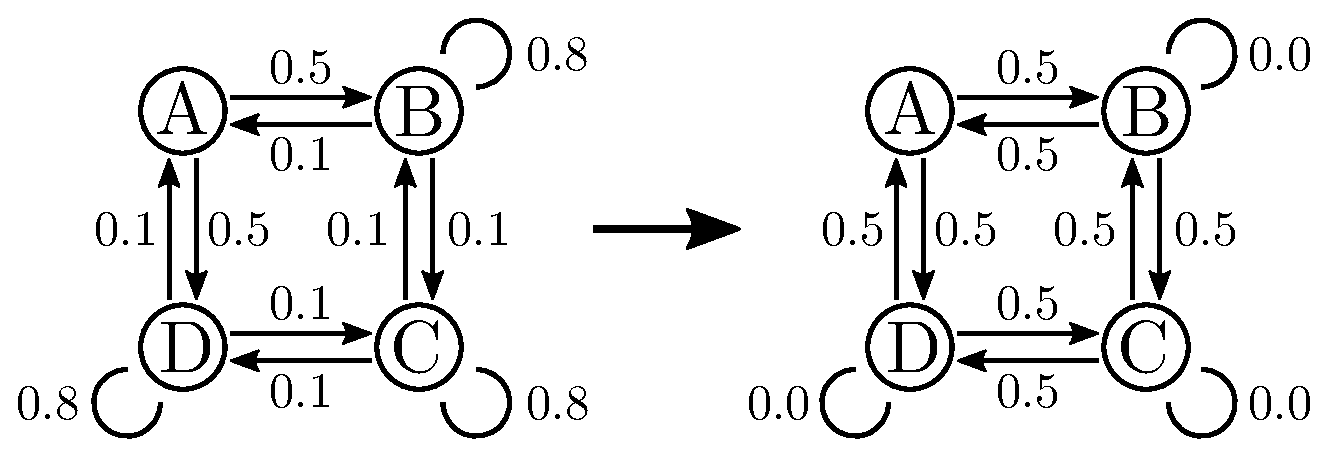
\includegraphics[width=\textwidth]{results/mc3_models}
        \vspace{-25pt}
        \caption{Model series III}
        \label{fig:mc3-models}
    \end{subfigure}
    \begin{subfigure}{0.85\textwidth}
    	\centering
        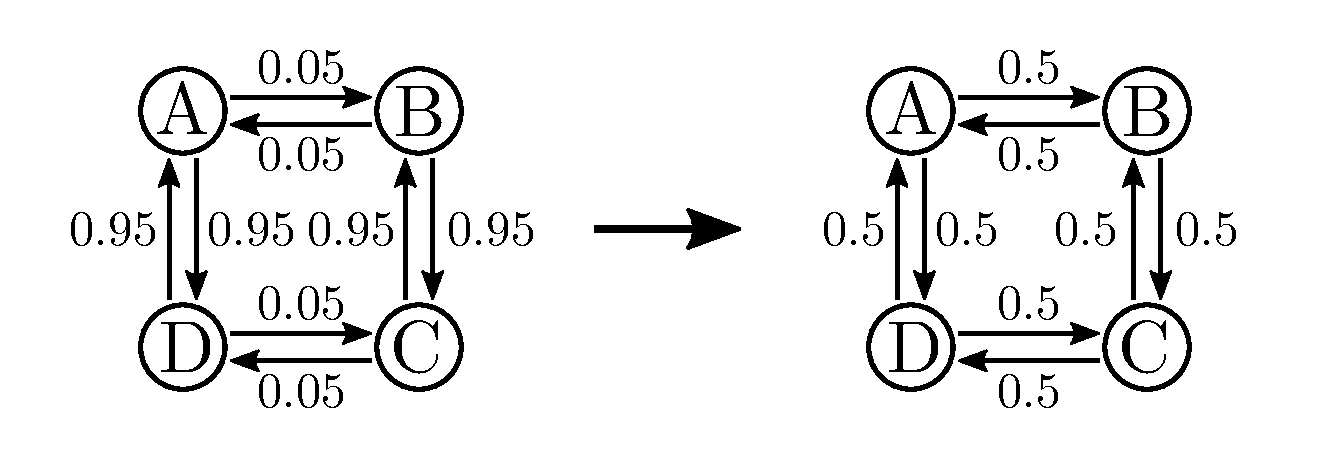
\includegraphics[width=\textwidth]{results/mc4_models}
        \vspace{-30pt}
        \caption{Model series IV}
        \label{fig:mc4-models}
    \end{subfigure}
    \begin{subfigure}{0.85\textwidth}
    	\centering
        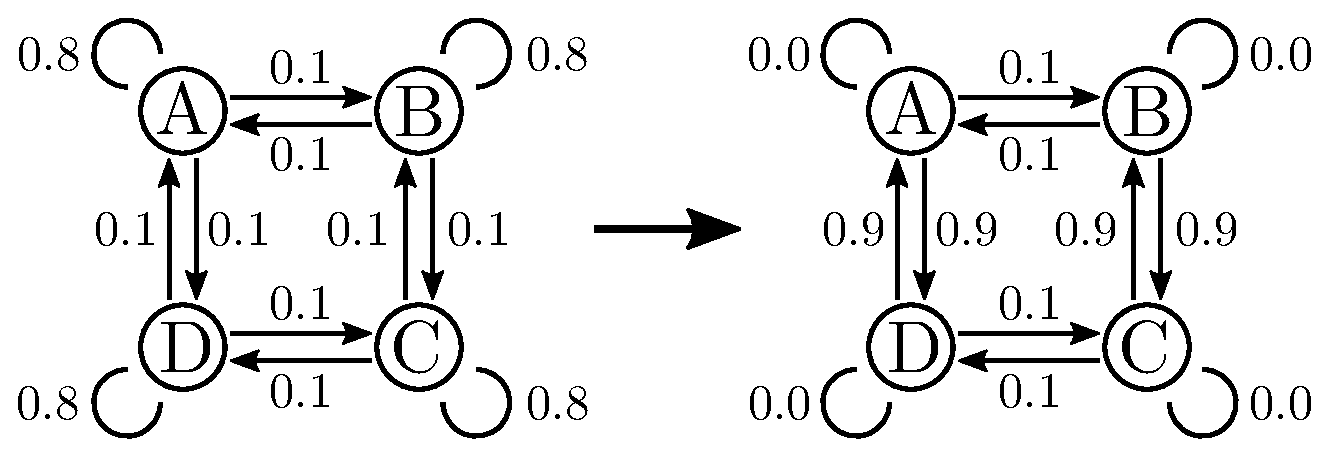
\includegraphics[width=\textwidth]{results/mc5_models}
        \vspace{-25pt}
        \caption{Model series V}
        \label{fig:mc5-models}
    \end{subfigure}
    \begin{subfigure}{0.85\textwidth}
    	\centering
        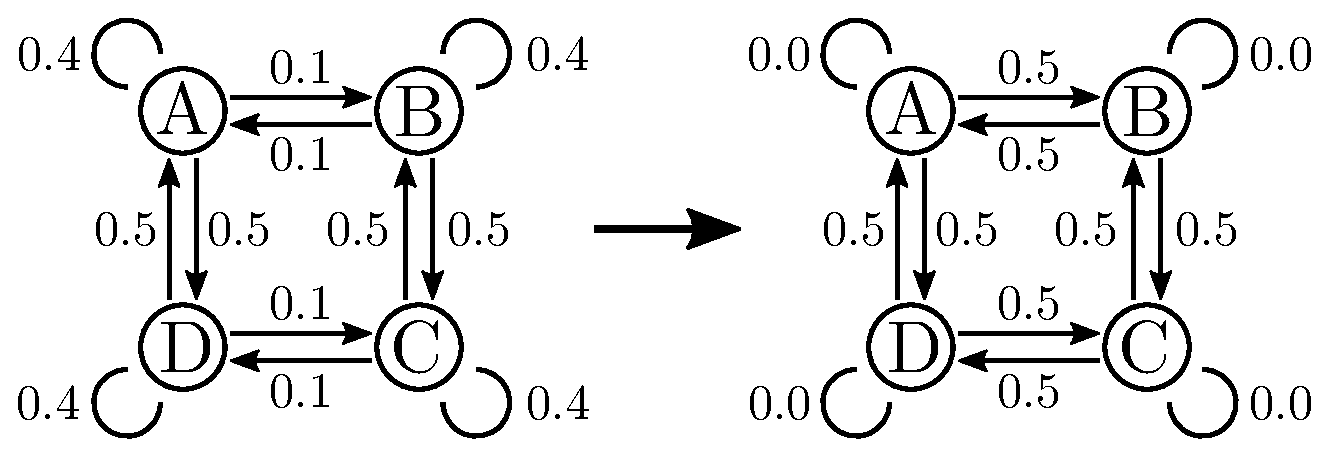
\includegraphics[width=\textwidth]{results/mc6_models}
        \vspace{-25pt}
        \caption{Model series VI}
        \label{fig:mc6-models}
    \end{subfigure}
    \caption[Four Markov model series to test the IP-hypothesis]{Four Markov model series to test the \acs{ip}-hypothesis. The first series in \textbf{a)} prefers state $B$, $C$ and $D$. Model by model, the self loop is decreasing and the probability to reach $A$ is increased. \textbf{b)} starts with a model which separates between the left and the right side. Series \textbf{c)} starts with a model where all four states are separated and changes step by step to a model where the right and left side are separated, which was the starting point in \textbf{b)}. Finally, in \textbf{d)} the first model separates between right and left and has some self loops additionally. This equals a middle model from \textbf{c)}. In series \textbf{b)}, \textbf{c)} and \textbf{d)} all models have the same stationary distribution with equal probability for every state.}
    \label{fig:mc-models-collection}
\end{figure}

\begin{figure}[p]
    \centering
    \begin{subfigure}{0.48\textwidth}
    	\centering
        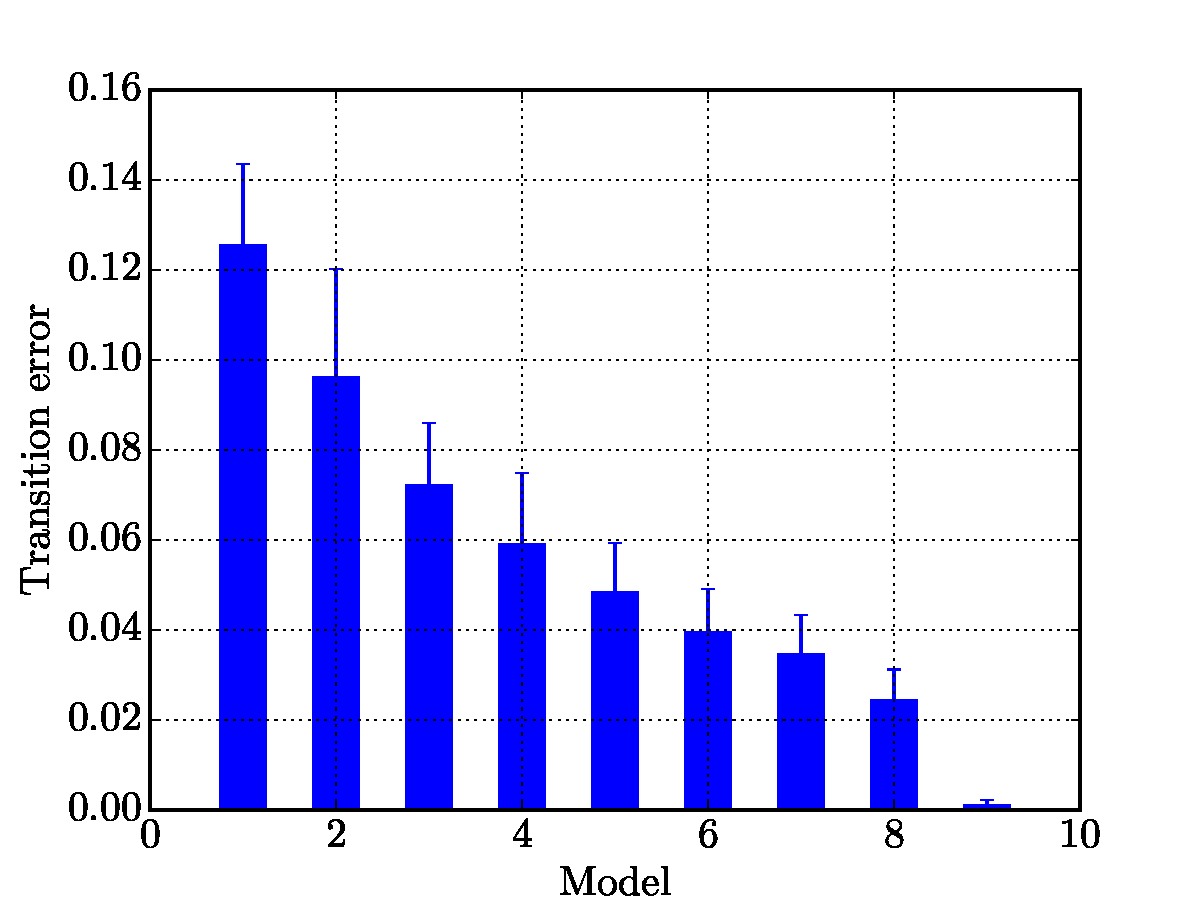
\includegraphics[width=\textwidth]{results/mc3_performance_distances}
        \caption{Model series III}
        \label{fig:mc3-performance-distance}
    \end{subfigure}
    \hfill
    \begin{subfigure}{0.48\textwidth}
    	\centering
        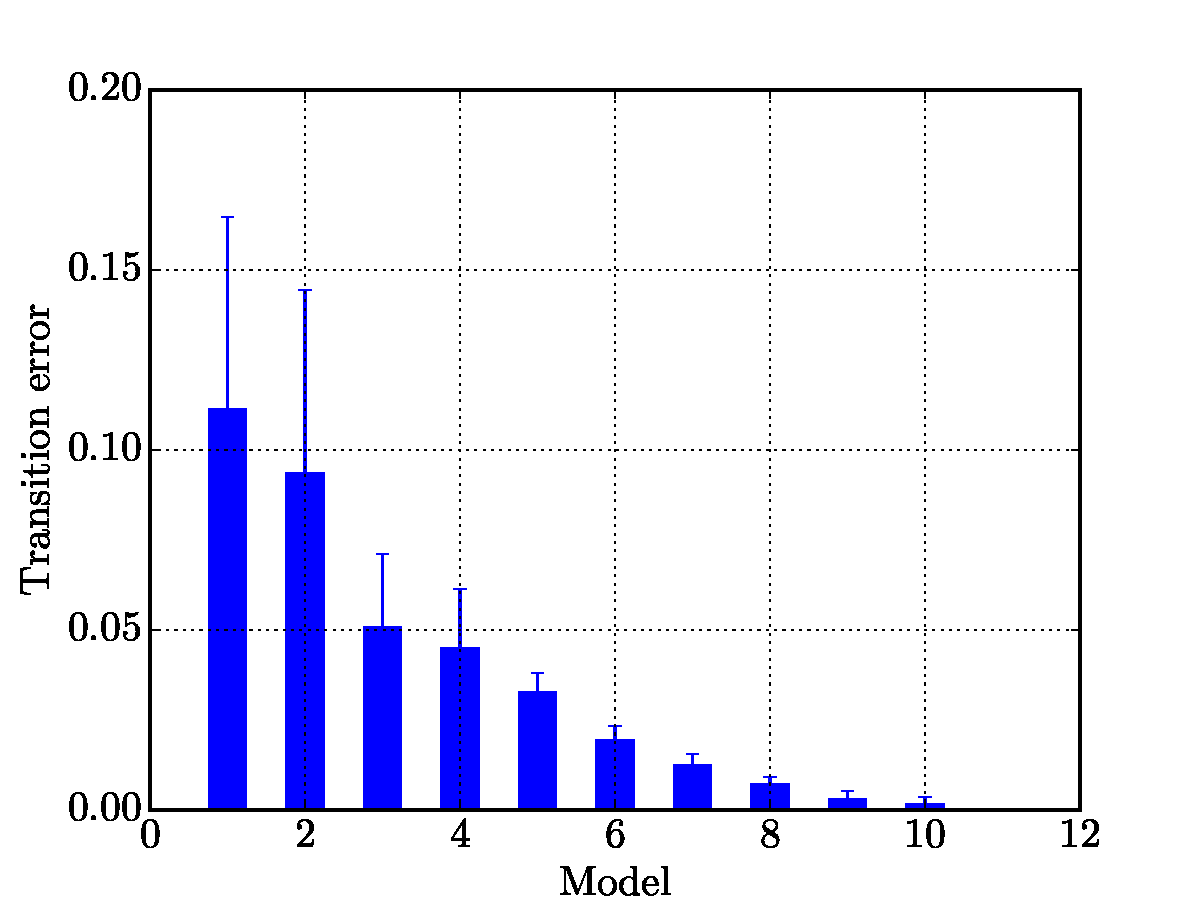
\includegraphics[width=\textwidth]{results/mc4_performance_distances}
        \caption{Model series IV}
        \label{fig:mc4-performance-distance}
    \end{subfigure}
    \begin{subfigure}{0.48\textwidth}
    	\centering
        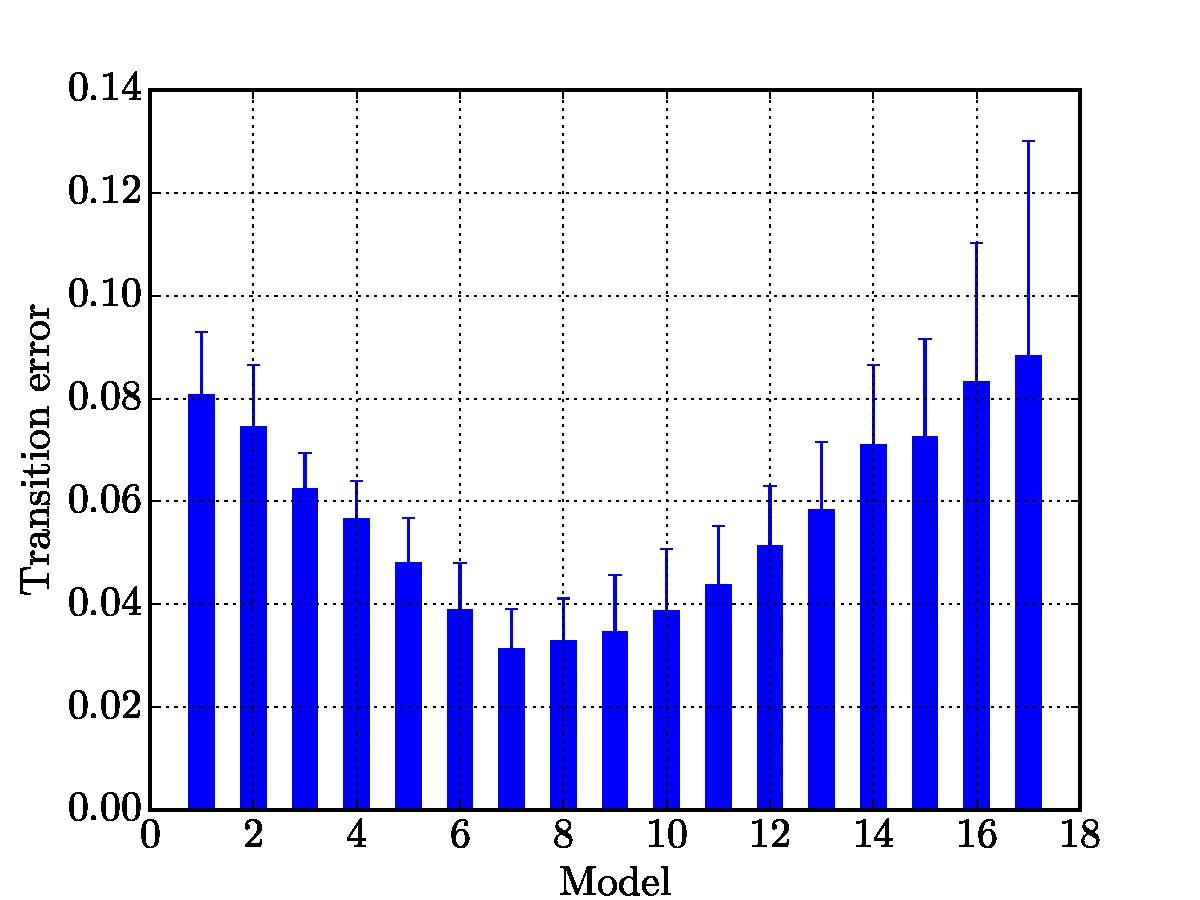
\includegraphics[width=\textwidth]{results/mc5_performance_distances}
        \caption{Model series V}
        \label{fig:mc5-performance-distance}
    \end{subfigure}
    \hfill
    \begin{subfigure}{0.48\textwidth}
    	\centering
        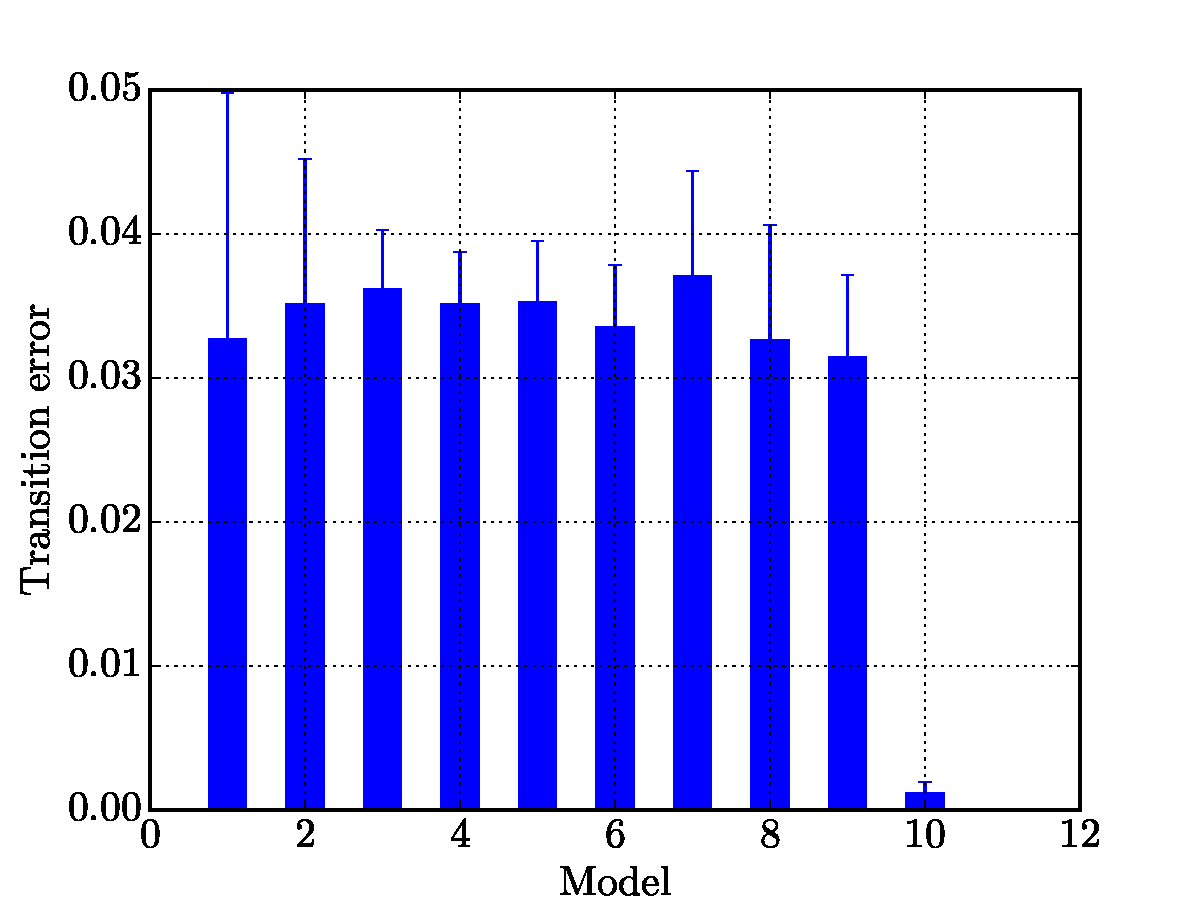
\includegraphics[width=\textwidth]{results/mc6_performance_distances}
        \caption{Model series VI}
        \label{fig:mc6-performance-distance}
    \end{subfigure}
    \caption[Performance of four Markov model series]{Performance of the four Markov model series from figure \ref{fig:mc-models-collection}. Model series III was divided into $9$ models, model series IV into $11$ models, model series V into $17$ models and model series VI into $11$ models. All four series follow the predicted behavior according to the \acs{ip}-hypothesis. The variance, the Kullback-Leibler divergence and the Gini coefficient, do not hold for prediction in cases \textbf{b)}, \textbf{c)} and \textbf{d)}, since every information and concentration measure is equal within every model series, while the performance differs significantly.}
    \label{fig:mc-series-performance}
\end{figure}

Model series IV, shown in figure \ref{fig:mc4-models}, separates the states $A$ \& $D$ and $B$ \& $C$ and join them step by step again. The interesting aspect of this approach is that the stationary distribution is absolutely equal for every model in this series, such that $\bm\pi = \left( \frac{1}{4}, \frac{1}{4}, \frac{1}{4}, \frac{1}{4} \right)^T$. At that point the predictors, namely the variance, Kullback-Leibler divergence and Gini coefficient, are the same for every model and would predict no differences in performance. On the other hand, the \acs{ip}-hypothesis predicts a change in performance. In the beginning, the probability to switch between the right and the left side is very small. Therefore, if one side is active, the chance increases that the other side will be active spontaneously. The more both sides are connected again, the better the performance should become. Figure \ref{fig:mc4-performance-distance} shows a clear decay in the \acs{mse} $\varepsilon_M$, which strongly supports the \acs{ip}-hypothesis. The down side of this result is, that the information and concentration measures do not longer hold as predictors. The information, contained in the stationary distribution is obviously not sufficient to predict the behavior.

Series V is more complex. In figure \ref{fig:mc5-models} the construction of the models is shown. It starts with a model where all four states are quite disconnected. It is expected that the performance is low in this case. The last model of this series equals the first model of the previous series. The model transforms from four separated parts to two separated parts. Comparing the performance of the first models and the last models in figure \ref{fig:mc4-performance-distance}, the error is quite similar. Therefore, it seems not very important if the chain is separated in four parts or in two parts. It seems to be more important how strongly the different parts are connected. Interestingly for the middle part, the error decreases. The middle model has a probability of $p_{x_i x_i} = 0.4$ for the self loop and $p_{AD} = p_{BC} = 0.4$. Probably the self loop increases the probability that the states can change between the right and the left side, since in some cases it stays in the same state and has another chance to switch. The first model suffers from a strong disconnection between all states. For those `islands' the self loop is not helpful. The last model has no self loops any more, which separates the the sides, as it was observed in the model series above. Note that the stationary distributions are the same for all models again, where each state has equal probability.

The last example, model series VI, is shown in figure \ref{fig:mc6-models} and again, all models in this series have the same distribution as before. In this case, the first model starts, where the third series was in its middle. At that point the performance was relatively good. The last model was already used before in many cases and is already known as a model which can be learned with high precision. It is predicted from what was observed before, that the self loop in the first models increase the probability that the states can switch the sides. The more the self loop probability is decreased, the more the direct connection between the two sides increase at the same time. This behavior should compensate the decrease in the self loops. It should result in a relatively similar performance for all models. Indeed, figure \ref{fig:mc6-performance-distance} shows that all models have a relatively constant and low error, where the last model is a little bit outstanding. Comparing this outlier model for example with \ref{fig:mc3-performance-distance}, indicates that this effect already happened before. A possible explanation is given in appendix \ref{sec:appendix:close}.

In conclusion, the \acs{ip}-hypothesis holds for all tested model series. In the following, the implementation of the \acl{ip} mechanism from equation \eqref{eq:hip-ind} is tested for different parameters to come closer to an understanding of how \acs{ip} works.

\paragraph{Influence of parameter $\bar H^\IP$}

\begin{figure}[!t]
    \centering
    \begin{subfigure}{0.48\textwidth}
    	\centering
        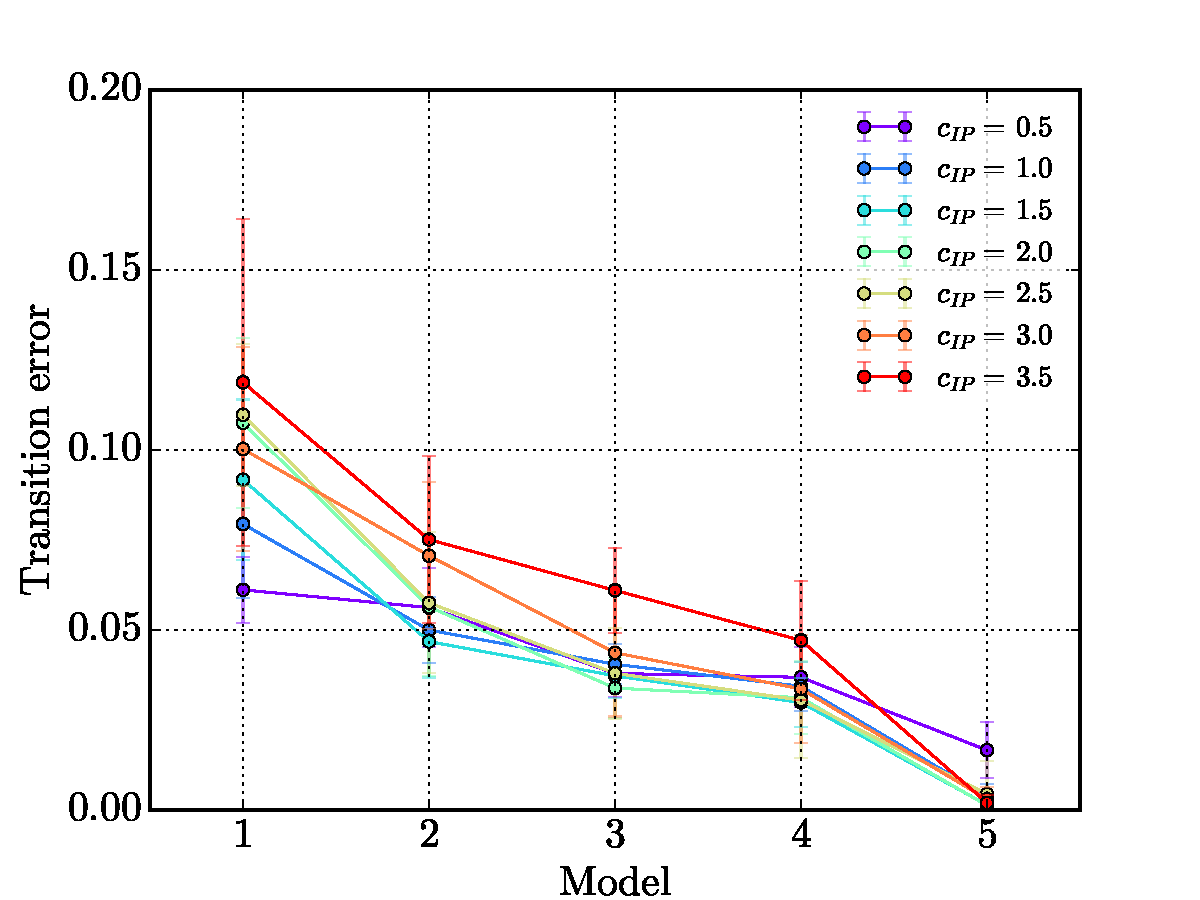
\includegraphics[width=\textwidth]{results/h_ip}
        \caption{}
        \label{fig:hip-allmodels}
    \end{subfigure}
    \hfill
    \begin{subfigure}{0.48\textwidth}
    	\centering
        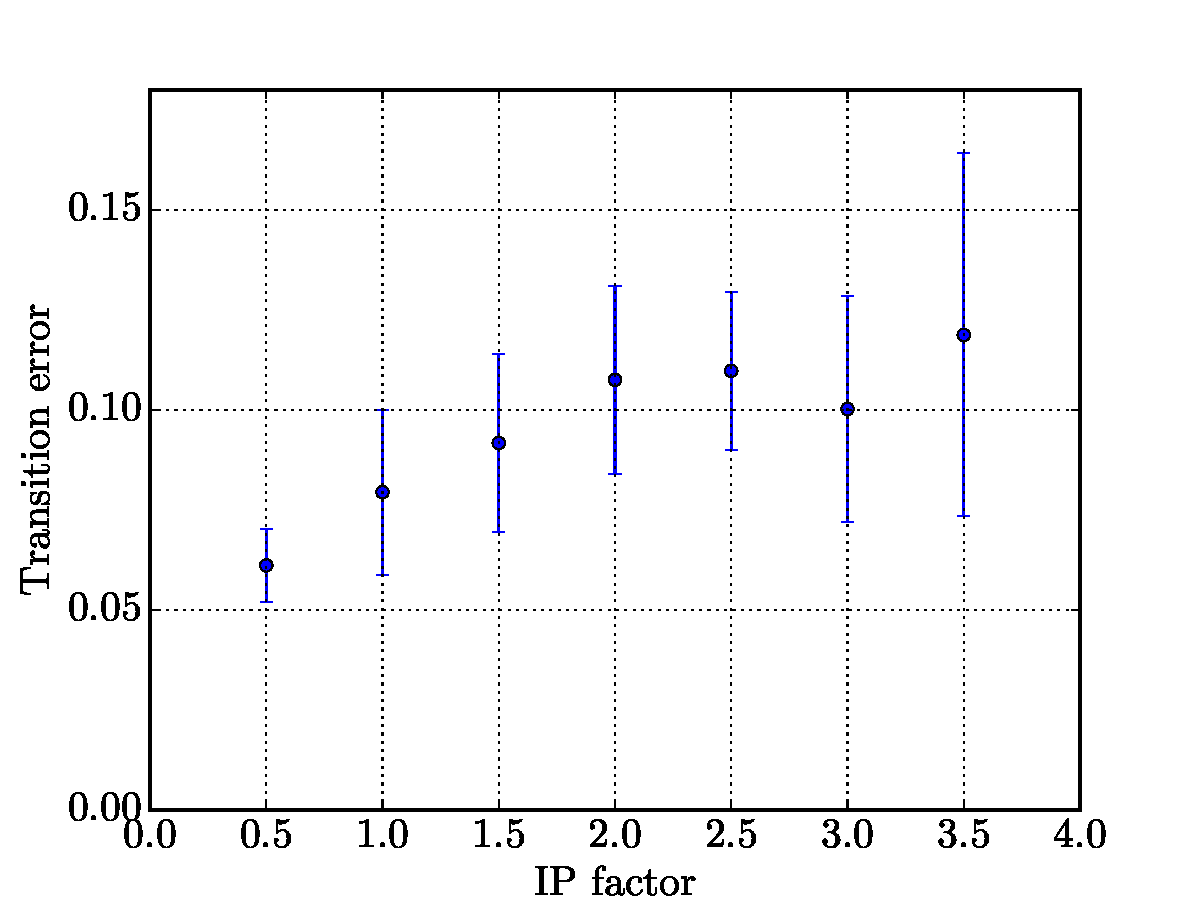
\includegraphics[width=\textwidth]{results/h_ip_model1}
        \caption{}
        \label{fig:hip-model1}
    \end{subfigure}
    \begin{subfigure}{0.48\textwidth}
    	\centering
        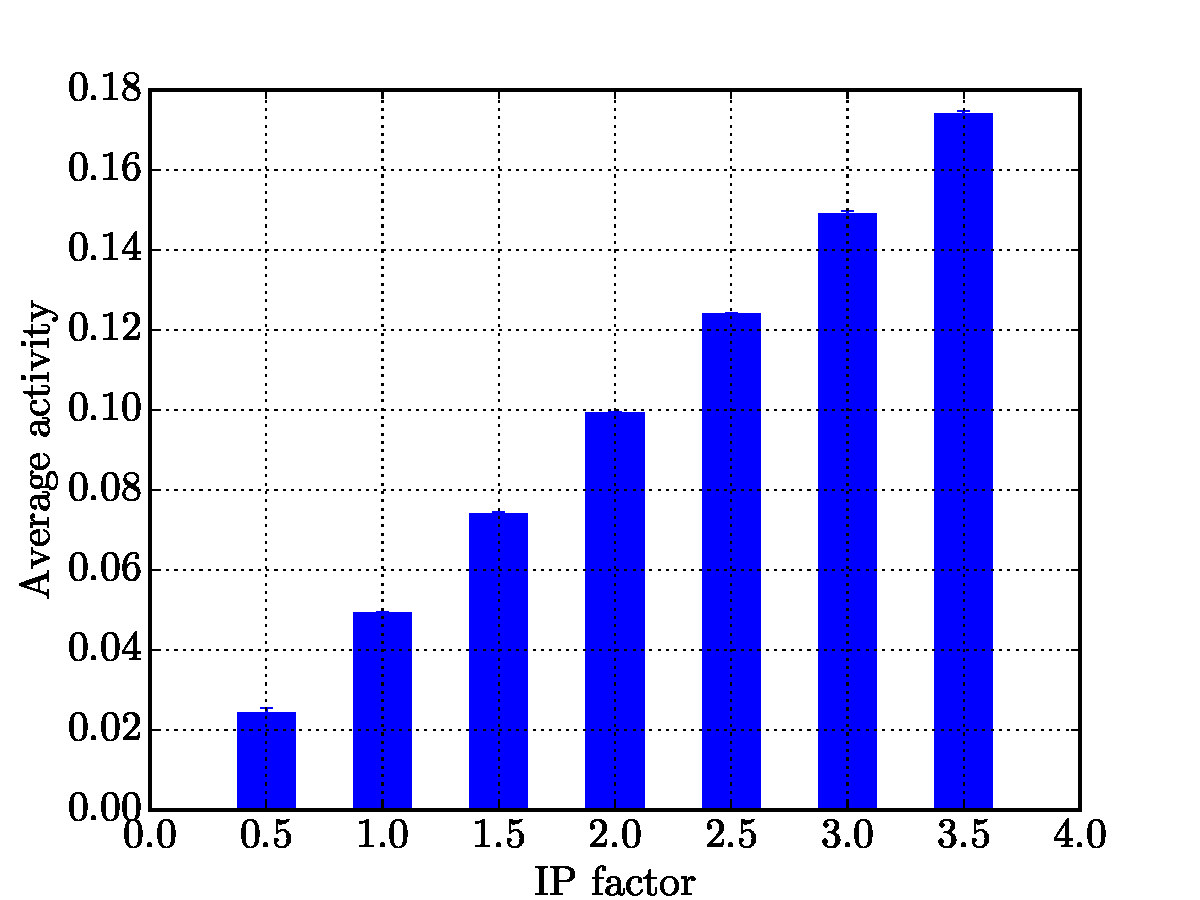
\includegraphics[width=\textwidth]{results/h_ip_activity_model1}
        \caption{}
        \label{fig:hip-activity-model1}
    \end{subfigure}
    \hfill
    \begin{subfigure}{0.48\textwidth}
    	\centering
        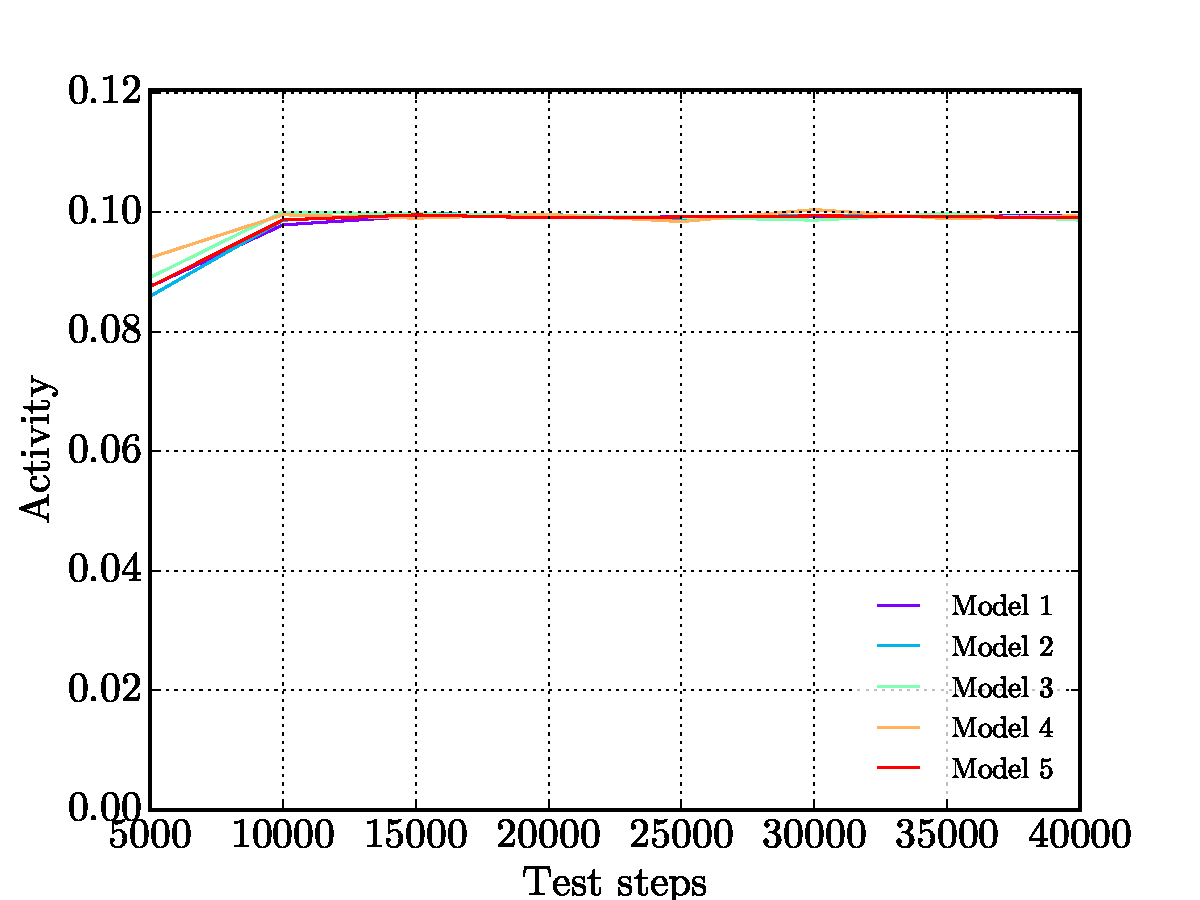
\includegraphics[width=\textwidth]{results/h_ip_test_traces_activity}
        \caption{}
        \label{fig:hip-activity-trace}
    \end{subfigure}
    \caption[Influence of the IP target rate]{Influence of the target rate on model series II, divided into $5$ models. The target rate factor $c_\IP$ was varied from $0.5$ to $3.5$ in steps of $\Delta c_\IP = 0.5$. \textbf{a)} shows the behavior for all models, where the performances of the first models seem to be influenced by the target rate. In \textbf{b)} a further investigation of the very first model was done, since effects are expected to be most clear for that model. It shows that the target rate has an effect on the performance for that model, where $p$-values are given in table \ref{tb:hip-ttests}. The average activity of the network for the first model is plotted in \textbf{c)}, showing that the target rate directly influences the activity in the network. In plot \textbf{d)} the activity for $c_\IP = 2.0$ is shown over the whole testing phase for all models. After a short burn in phase, the activity stays very constant. Note that this plot bases only on a single simulation. In all cases, errorbars indicate standard errors.}
    \label{fig:hip-influence}
\end{figure}

If the \acl{ip} is responsible for the performance differences between the models, then a change of the parameters of the \acs{ip} mechanism should be reflected in the performance of the models. $\bar H^\IP = 2\cdot N^U/N^E$ is the main factor inducing spontaneous activity. The lower the target rate $\bar H^\IP$, the less spontaneous activity is present and vice versa. Models, where specific states are less probable, should profit from a lower target rate. Those states can stay silent for a longer time until \acl{ip} will spontaneously activate them. Since the \acs{ip} is the only source for activity in the testing phase, it is somehow problematic to change the parameter. The \acs{ip} mechanism directly changes the average activity in the network. It cannot be excluded that it is the activity level in general rather than the threshold of the mechanism which influences changes in performance. For the simulation a parameter $c_\IP$ was used, such that $\bar H^\IP = c_\IP \cdot N^U/N^E$ where $c_\IP = 2$ is the default value.

However, the results with different $c_\IP$ values are shown in figure \ref{fig:hip-influence}. It was applied to the systematic model series II from figure \ref{fig:mc2-models}. For simplicity of the presentation of the results in the plots, the series was created with just $5$ models in opposite to results shown in figure \ref{fig:mc2-kl}, where the series was applied with $9$ models. The first plot in figure \ref{fig:hip-allmodels} shows the performance of all $5$ models and all $c_\IP$ values. As expected from the results before, the error decreases when state $A$ is less isolated. In those models, where state $A$ is highly isolated, the \acs{ip} target rate influences the performance of the models. For evaluation, the first model was chosen. This model has the lowest probability to reach state $A$ and therefore the target rate should have the highest influence to that model. In figure \ref{fig:hip-model1} the performance results for the first model are shown, depending on the \acs{ip} factor $c_\IP$. It seems that there is a positive correlation between the parameter and the error $\varepsilon_M$, at least between $c_\IP = 0.5$ and $c_\IP = 2.0$. In table \ref{tb:hip-ttests}, t-tests between all errors value were applied, showing that the intuition is correct. The main effect happens before $c_\IP = 2.0$, afterwards no significant changes can be observed. This results supports the \acs{ip}-hypothesis, even though the effects seem to decay very fast with further models.

\begin{table}[!t]
\centering
\begin{tabular}{c|ccccccc}
$c_\IP$ & $1.0$ & $1.5$ & $2.0$ & $2.5$ & $3.0$ & $3.5$ \\
\hline
$0.5$ & \makecell{$\mathbf{1.08\cdot 10^{-3}}$\\ \starsSS} & \makecell{$\mathbf{2.46\cdot 10^{-6}}$\\ \starsSSS} & \makecell{$\mathbf{1.12\cdot 10^{-9}}$\\ \starsSSS} & \makecell{$\mathbf{6.61\cdot 10^{-12}}$\\ \starsSSS} & \makecell{$\mathbf{1.37\cdot 10^{-6}}$\\ \starsSSS} & \makecell{$\mathbf{3.44\cdot 10^{-6}}$\\ \starsSSS} \\
$1.0$ & & \makecell{$0.085$\\ \starsNS} & \makecell{$\mathbf{3.62\cdot 10^{-4}}$\\ \starsSSS} & \makecell{$\mathbf{4.01\cdot 10^{-5}}$\\ \starsSSS} & \makecell{$\mathbf{0.014}$\\ \starsS} & \makecell{$\mathbf{1.41\cdot 10^{-3}}$\\ \starsSS} \\
$1.5$ & & & \makecell{$\mathbf{0.040}$\\ \starsS} & \makecell{$\mathbf{0.011}$\\ \starsS} & \makecell{$0.310$\\ \starsNS} & \makecell{$\mathbf{0.025}$\\ \starsS} \\
$2.0$ & & & & \makecell{$0.750$\\ \starsNS} & \makecell{$0.395$\\ \starsNS} & \makecell{$0.343$\\ \starsNS} \\
$2.5$ & & & & & \makecell{$0.236$\\ \starsNS} & \makecell{$0.433$\\ \starsNS} \\
$3.0$ & & & & & & \makecell{$0.139$\\ \starsNS} \\
\end{tabular}
\vspace{5pt}
\caption[p-values of performance differences between $\bar H^\IP$ values]{$p$-values of performance differences for simulations with different target rate factors $c_\IP$ for model $1$. Bold values indicate significant differences with $p \le 0.05$.}
\label{tb:hip-ttests}
\end{table}

Figure \ref{fig:hip-activity-model1} shows the average activity for the first model, depending on the target rate. It is clear from that plot that $\bar H^\IP$ directly influences the amount of activity, which is defined as the number of spiking excitatory neurons $n_{\text{spiking}}(t) = |\ \{ i \in \{1, ..., N^E\} \,:\, x_i(t) = 1\} |$ divided by the total number of excitatory neurons $N^E$ at a specific point in time $t$. Additionally, for a fixed $c_\IP$, the activity is very stable and independent of the model, as shown in figure \ref{fig:hip-activity-trace}. It shows the activity over the testing phase for $c_\IP = 2.0$ for a single simulation. Note that this activity is not averaged. The activity differences could potentially influence the performance directly. To exclude effects from the amount of activity in the networks, noise could be implemented to hold a specific level of activity. This approach is considered in the discussion in section \ref{sec:discuss-ip}. 

However, even though the effects are not very strong and possibly influenced by the activity, in tendency, they support the \acs{ip}-hypothesis.

\paragraph{Influence of parameter $\sigma^\IP$}

\begin{figure}[!b]
	\centering
	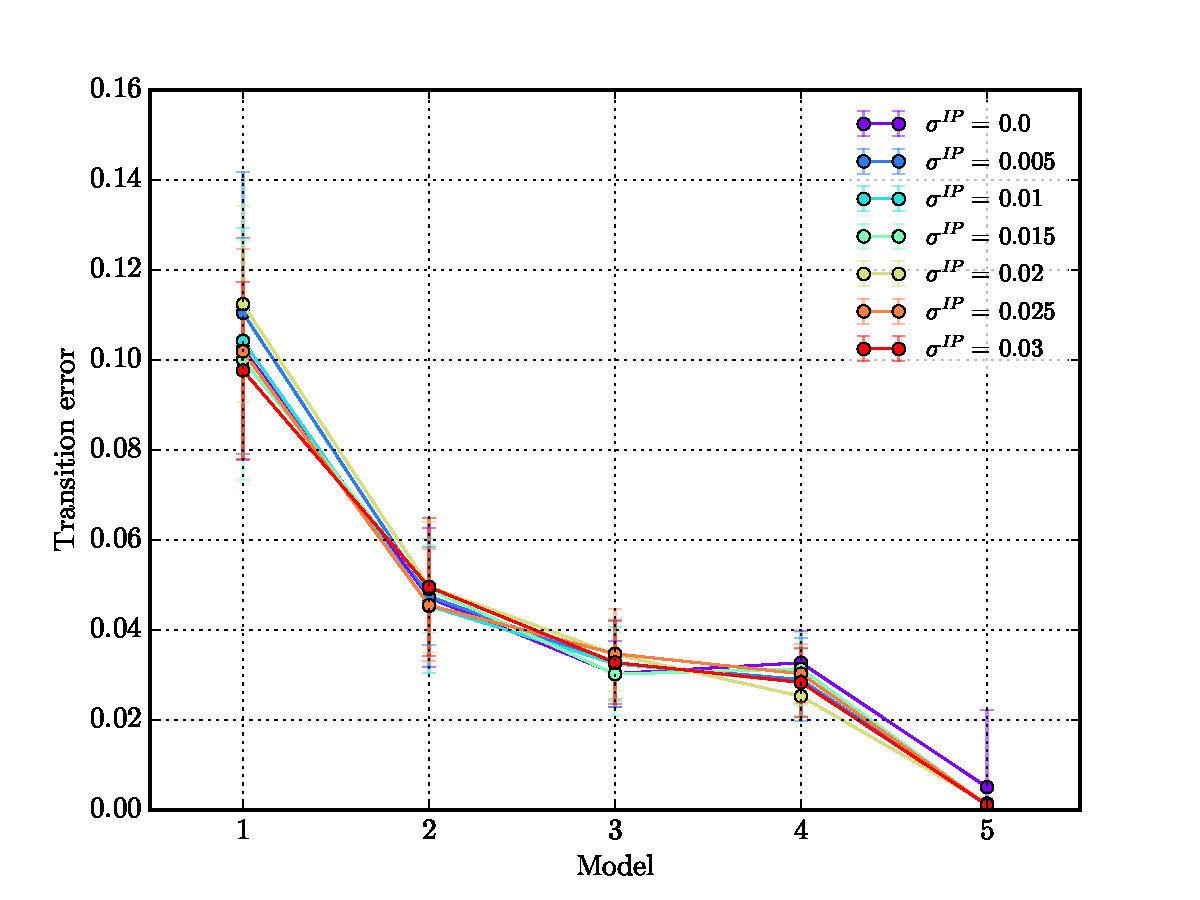
\includegraphics[width=0.85\textwidth]{results/h_ip_range}
	\caption[Influence of the IP target rate range]{Variation of \acs{ip} target rate range $\sigma^\IP$ applied to model series II, divided into $5$ models. The target rate range was varied from $0.0$ to $0.03$ with steps of $\Delta \sigma^\IP = 0.05$. Error bars indicate standard errors. The performance is independent from the chosen target rate range for all models.}
	\label{fig:hip-range}
\end{figure}

\textcite{hartmann2015s} have shown that the network performs more robust if the target rate is not the same for every neuron. Therefore, in this thesis the parameter $\sigma^\IP$ was introduced in section \ref{sec:ip-mod} and chosen as $0.01$, pursuant to their suggestion. The parameter determines the range, how much a target rate of a specific neuron can differ from the average target rate $\bar H^\IP$. According to \textcite{hartmann2015s}, the performance should decrease if $\sigma^\IP$ is lower than $0.01$ or even zero. The latter case with $\sigma^\IP = 0$ corresponds to the rule \textcite{lazar2009sorn} used in the initial \acs{sorn}. Beside reproducing the behavior for $\sigma^\IP < 0.01$, it also remains to show what happens if $\sigma^\IP$ is increased above $0.01$ and to evaluate the results in context of the \acs{ip}-hypothesis.

To keep it comparable with the variation of the $\bar H^\IP$ parameter, also the systematic model series II from figure \ref{fig:mc2-models} was applied, divided into $5$ models. Figure \ref{fig:hip-range} shows the  performance of all $5$ models for all $\sigma^\IP$ values. The differences in the performance are not significant ($p > 0.05$) for all models, except one, where the difference between $\sigma^\IP = 0.02$ and $\sigma^\IP = 0.03$ in the first model is significant with $p = 0.035$. But since the significance level is low and all other $20$ comparisons for the first model alone are non-significant, the results from \textcite{hartmann2015s} could not be reproduced. Contrary to their findings, the present findings suggest no effect below $\sigma^\IP < 0.01$, nor is an effect above $\sigma^\IP > 0.01$. The result suggests that the initial \acs{ip} rules from \textcite{lazar2009sorn} is sufficient. Regarding the \acs{ip}-hypothesis, the $\sigma^\IP$ parameter seems to have no or at best a very small influence on the less probable states. Since the arguments of \textcite{hartmann2015s} for introducing $\sigma^\IP$ are plausible, perhaps further research is necessary to understand in which cases a variation of the parameter for the neurons can increase the robustness. A suggestion for another approach is given in the discussion section, in subsection \ref{sec:discuss-ip}.

\paragraph{Other parameters}

Two other aspects should be considered: the learning rate $\eta_\IP$ and the connectivity of the network.

First, $\eta_\IP$ is the learning rate of the \acl{ip}. The higher the learning rate, the faster the network reaches its target rate $\bar H^\IP$. It should not influence the performance of the models, since the burn in phase was always excluded from evaluation. However, the effect of $\eta_\IP$ regarding the burn in phase is considered in appendix \ref{sec:appendix:eta}.

Beside effects from the \acl{ip}, it is also necessary that the neurons are adequately connected. It could be that this assumption does not hold. Under some conditions, the structure of the network may be rather good, under others rather bad. An approach to test if such effects possibly occur, is to vary the connectivity of the network. It is the average number of connections between the excitatory neurons, denoted by $\lambda^W = \rho \cdot N^E$, where $\rho = 0.1$ by default. If $\rho$ is changed, the number of average connections changes. According to the appendix section of \textcite{lazar2009sorn} a sparse network with about $10\%$ of connections performs best. It means that every neuron is connected with $10\%$ of the other excitatory neurons in the network. If the number of connections is too high, there is a higher risk that the activity in the network grows without bounds. In context of the \acs{ip}-hypothesis, it is probably worth to vary the connectivity $\rho$ again in the setting of the Markov chain approach. The results are shown in appendix \ref{sec:appendix:connectivity}. It was possible to reproduce former results and a connectivity of $10\%$ seems to fit well, also in context of the \acs{ip} hypothesis. If the connectivity is too low or too high, the error increases.



